%Article
\documentclass[10pt]{report}

%Standard thesis size
\usepackage[a4paper,left=3cm,right=2.5cm,top=3cm,bottom=3cm,]{geometry}

%comment large sections of text. 
\usepackage{comment}
% \begin{comment} 
% Commented text 
% \end{comment} 

%To make [H] Work
\usepackage{float}

%Loading comment package 
\usepackage{comment}

% for fancy looking tables
\usepackage{booktabs}   

%This package slashes dirac operators 
\usepackage{slashed}

% Good old Checkmarks
\usepackage{pifont}

%Not sure
\usepackage[english]{babel}

% References I'd guess 
\usepackage{hyperref} 
%\usepackage{apacite} 

%Mathematical expressions 
\usepackage{amsmath}
\usepackage{amssymb}

% Where are the images
\usepackage{graphicx}
\graphicspath{{./Images/}}

% inputs 
\usepackage[utf8]{inputenc}

%Using Sub files
%Perfect comment Pedro, cat --> this says cat
\usepackage{subfiles}

%images in here 
\graphicspath{{./Images/}}

%Horizontal line
\usepackage{cancel}

%tables 
\usepackage{tabularx}

%using a colored text 
\usepackage{xcolor}

\newcommand{\ro}[1]{\textrm{#1}}
\newcommand{\U}[1]{\mathrm{U}(1)_{\mathrm{#1}}}
\newcommand{\Z}[1]{\mathrm{Z}(1)_{\mathrm{#1}}}			
\newcommand{\SU}[1]{\mathrm{SU}(2)_{\mathrm{#1}}}			

% Thesis format
\usepackage[DF,newLogo]{uaThesis}
\setlength\extrarowheight{2pt}
	
% optional: visual delimiters for floats (figures and tables)
\def\topfigrule{\kern 7.8pt \hrule width\textwidth\kern -8.2pt\relax}
\def\dblfigrule{\kern 7.8pt \hrule width\textwidth\kern -8.2pt\relax}
\def\botfigrule{\kern -7.8pt \hrule width\textwidth\kern 8.2pt\relax}

%nova pagina ao fim da seção
\usepackage{titlesec}
\newcommand{\sectionbreak}{\clearpage}

%\renewcommand{\cftsecfont}{\rmfamily\mdseries\upshape}
%\renewcommand{\cftsecpagefont}{\rmfamily\mdseries\upshape} % No bold 
%\usepackage{apacite}
\def\ThesisYear{2020}

% Added in November 
\usepackage{flexisym} % This package allows me to use a Prime in text format 

%Shamelessly stolen, this makes life so much easier 
\renewcommand{\(}{\left(}

\renewcommand{\)}{\right)}

\renewcommand{\[}{\left[}

\renewcommand{\]}{\right]}

%check marks
\newcommand{\cmark}{\ding{51}}%
\newcommand{\xmark}{\ding{55}}%

\begin{document}


\TitlePage
  \HEADER{\BAR\FIG{\includegraphics[height=60mm]{uaLogoNew.pdf}}} 
%	
  {\ThesisYear}
  \TITLE{ João Pedro Dias Rodrigues }
        { A Study of possibilities beyond the Standard Model}
\EndTitlePage
\titlepage\ \endtitlepage % empty page

\TitlePage
  \vspace*{55mm}
  \TEXT{\textbf{o j\'uri~/~the jury\newline}}
       {}
  \TEXT{presidente}
       {\textbf{Margarida Facão}\newline {\small
        Professora Auxiliar do Departamento de Física da Universidade de Aveiro}}
  \vspace*{5mm}
  \TEXT{vogais}
       {\textbf{António Morais}\newline {\small Investigador Pos-doc do Departamento de Física da Universidade de Aveiro}}
  \vspace*{5mm}
  \TEXT{}
       {\textbf{Nuno Castro?}\newline {\small
        Professor at the University of Minho. Researcher at LIP and ATLAS experiment at CERN. }}
  \vspace*{5mm}
\EndTitlePage
\titlepage\ \endtitlepage % empty page

\TitlePage
  \vspace*{55mm}
  \TEXT{\textbf{agradecimentos~/\newline acknowledgements}}
       {Honestamente acho que isto vai ter que ser escrito antes da entrega }
  \TEXT{}
       {Honestly this will be written in english translated poorly from above :) }
\EndTitlePage
\titlepage\ \endtitlepage % empty page

\TitlePage
  \vspace*{55mm}
  \TEXT{\textbf{Resumo}}
       {É impossível debater que o surpreendente sucesso do modelo padrão de física de partículas o faz um dos maiores sucesso da ingenuidade humana, no entanto, apesar de o modelo padrão descrever com grande detalhe todas as partículas observadas e as suas interações e conseguir tratar um grande número de fenomeno  físicos onde era esperado encontrar falhas, tudo numa estrutura bem motivada, este é considerado incompleto. \\ { \color{green} 
Introduzir motivação para a falha do SM. \\
Introduzir motivação para mais Higgs. \\ 
Introduzir motivação para o BLSM \\ 
Introduzir motivação para o 3HDM} \\ 
{\color{blue} Tocar nas conclusões?? }
       }
\EndTitlePage
\titlepage\ \endtitlepage % empty page

\TitlePage
  \vspace*{55mm}
  \TEXT{\textbf{Abstract}}
       {
       This part will be in English. Translated from above. 
       }
\EndTitlePage
\titlepage\ \endtitlepage % empty page


\pagenumbering{roman}
\tableofcontents

\cleardoublepage
\listoffigures

\cleardoublepage
\listoftables

\cleardoublepage

\pagenumbering{arabic}
\setcounter{page}{1}

\section{Labels}

{{\color{green}A paragraph or text to be added later  }

{{\color{red}   A mistake or a question that is likely wrong }

{{\color{blue}  A comment or doubt to ask or check}

{{\color{gray} Excess? Probably will cut, waiting for advice} 

%%\chapter{Introduction}
%\label{ch:Intro}

\newpage

\chapter{Introduction}
\label{chapter:Introduction}
%\section{Introduction}

%\section{The Sturdy SM with some holes}

\Joaorep{The modern study of particle physics}{Our current understanding of all subatomic phenomena} must be \Joaorep{taught}{understood} trough the Standard Model (SM) of particle physics. 
%
The SM has thus far \Joaoadd{been} the best descriptor for the experimentally observed spectra of particles and their interactions at \Joaorep{all current probable scales}{the electroweak (EW) scale}. 
%
And \Joaorep{In}{in} 2012\Joaoadd{,} a resonance was discovered \Joaorep{in}{at} the \Joaorep{LHC}{Large Hadron Collider (LHC)} that seems to confirm the existence of \Joaorep{it's}{its} last predicted particle, the Higgs boson, finally completing the model and proving the existence of the Higgs mechanism \cite{Aad_2012,chatrchyan2012observation,
collaborations2015combined,collaborations2016measurements} \Joao{Não necessitas de tantas referências para o Higgs, uma ou duas basta}. 

The development of the SM was a arduous task, it led scientists  \Joaoadd{to} successfully combine three of the four fundamental forces of nature in a \Joaoout{very} well motivated framework, making it one of the most monumental achievements in theoretical physics.
%
However, despite \Joaorep{it's}{its} successes the SM still lacks a strong explanation for several experimental observations. \Joaoout{They have become more numerous by the decade, and to provide a "short" overview of some of them.}

\Joaorep{We firstly}{First, we} have the fact \Joaoadd{that} the SM can not account for one of the most important cosmological discoveries of the century, the existence of dark matter \Joao{Ref.}. This is a fundamental flaw since the SM lacks a possible dark matter candidate, or dark particle \Joao{Ref.}. 
%
Secondly, the SM lacks any justification for the existence of baryon asymmetry in the universe \Joao{Ref.}, i.e. why is the universe primarily made of matter rather than anti-matter. 
%
Although, \Joaoout{note that} the Electroweak baryogenesis (EWBG) remains a theoretically possible scenario for explaining the cosmic baryon asymmetry \Joao{Ref.}, a scenario viable in the SM framework.
%
Thirdly, the SM suffers from peculiar oddities in the fermion sector in the form of unjustified mass and mixing hierarchies. This is usually refereed to as the \Joaorep{\textit{flavour problem}}{flavour problem} and is considered a sizeable drawback of the SM .  
%
As \Joaorep{a}{an} example, we observe the top quark to be five order of magnitudes heavier \Joaoadd{than} the up quark , and eleven orders of magnitude than the observed neutrino masses \Joao{secalhar põe aqui os valores das massas, fica mais elucidativo, ou pelo menos, a ordem. Para o top $\mathcal{O}(100)$ GeV, o up $\mathcal{O}(1)$ MeV e os neutrinos $\mathcal{O}(1)$ eV}. These high differences are thought to be too large to be natural, so a physical property that would justify such gap is a desired property of most Beyond the Standard Model (BSM) frameworks. 
%
Fourth, \Joaoout{note} neutrino masses are not included in the SM. Although there are precise oscillation measurements \Joao{Ref.} that \Joaorep{measure}{estimate} masses in the eV range with precise mixing \Joaoout{in} between 3 different generations of neutrinos \Joao{Uma nota aparte, as oscilações dos neutrinos dependem da diferença de massas entre gerações $\Delta m$ e não da massa absoluta de cada um, ou seja, um deles pode não ter massa, mas um outro tem de ter}. 
%
There are still many other subtitle flaws, like the lack of a strong phase transition, \Joaoadd{the hiearchy problem, the $R_\kappa$ and g-2 anomalies,} etc.  \Joao{Mencionar pelo menos a anomalia g-2, pois analisas mais à frente no B-L-SM} 

These are just some of the typical justifications given to explore possible BSM scenarios. The holy grail of which would be a model that \Joaorep{include}{solves} all \Joaoadd{of} these problems in a properly motivated framework that addresses these and many more cosmological, gravitational \Joao{Gravitational? O que queres disser aqui? Não falas de gravidade quântica na tese.} and phenomenological problems.  
% 
For now\Joaoadd{,} such a model remains out of reach, so the narrowing down of theories through phenomenological studies is a very worthwhile endeavour. We try to present one of these studies in this work. % to the steady advancement of a more complete theory. 
%
Paradoxically \Joaoout{fortunately}, as of late\Joaoadd{,} these studies have become progressively harder to perform given that the available space for new physics \Joaoadd{(NP)} gets reduced by each successful particle experiment. 
%
Chief among \Joaorep{these experiments}{them} \Joaorep{is the}{are the CMS and ATLAS experiments at the} \Joaoout{Large Hadron Collider} LHC, whose large amount of collect data over past years is setting \Joaorep{more and more stringent}{ever stringent} bounds on viable parameter spaces of popular BSM scenarios. 
%
And as \Joaoadd{the} available space for \Joaorep{new physics}{NP} decreases\Joaoadd{,} it becomes more challenging to reveal \Joaoadd{the} remaining space without falling within the possibility of fine tuning our model.  

%{\color{blue} How to properly explain what fine tunning is? Should I?}

Note, that the SM has \Joaorep{shown increasingly}{increasingly shown} \Joaorep{consistence}{consistency} with most constraints that were initial believed to be a possible gateway to \Joaoout{new physics} NP or that would diverge from \Joaorep{it's}{its} predictions. Thus, the search continues for hints at possible directions to complete the SM. % One of these is brought to use trough flavour physics, as we'll soon examine further bellow. 

Conventionally, phenomenological simulations of BSM searches in these multi-dimensional parameter spaces have been made in large computer-clusters, \Joaorep{with use of}{requiring} several weeks of computational time trough \Joaorep{simple}{the use of} Monte-Carlo methods. 
%
Although this is the basis of the work presented here\Joaoadd{,} a effort was made to incorporate new machine learning routines \Joaorep{trough}{via} the initial building of smaller learning sets \Joaorep{trough}{by} conventional methods. 
%
Unfortunately this \Joaorep{wasn't}{was not} accomplished in this work due to the \Joaorep{expectational}{exceptional} setbacks. A feature of this year, that \Joaorep{affected partially}{partially affected} the quality of the work. 

\Joao{Como não fazes machine learning, acho que não te devias referir a isto.}

%%%% so far so good

During this \Joaorep{work}{thesis} we \Joaoout{shall} \Joaorep{do}{embark in} a small expedition into two possible BSM scenarios.
%
To achieve this, we will start by laying down the fundamental basis for this BSM discussion by presenting a short overview of the SM \Joaorep{, then we discuss possible extensions}{followed by a discussion into potential extensions of this framework.}\Joaoout{ to the SM}. \Joaorep{Namely, first by presenting}{First, we introduce} the B-L-SM model, a simple unitary extension based on a apparently accidental symmetry of the SM.  \Joao{Que simetria? Acho que ficava bem mencionar aqui}.
%
\Joaorep{And then by moving on}{Then, we move on} to a more complex model with additional Higgs doublets fields as \Joaorep{a}{an} attempt to present a framework that addresses the \Joaorep{\textit{flavour problem}}{flavour problem}. 
%
We will see how these \Joaoout{multiple doublet} \Joaorep{Models}{models} can address problems that \Joaoadd{a} simple unitarity extension \Joaorep{can't}{can not} and vice-versa. For example\Joaoadd{,} multiple Higgs \Joaorep{Doubles}{doublets} can easily offer \Joaorep{a}{an} explanation for the observed excess of charge parity or $\mathcal{CP}$ violation \Joaoadd{b}ut suffer from the possible inclusion of tree-level Flavour Changing Neutral Currents (FCNCs). These FCNCs are undesirable\Joaoadd{,} at least in large number\Joaoadd{,} given \Joaoadd{current} observations \Joao{Refs.}, so mechanisms have to be put in place to prevent them, while in the case of the simple unitary extensions such problems do not arise. 

%We will see how these models with more than one Higgs doublet can address yet another, thus far, unmentioned problem in the SM, the observed excess of charge parity or $\mathcal{CP}$ violation.  
%
%While suffering the possible the drawbacks of potentially having large Flavour Changing Neutral Currents (FCNCs). These FCNCs are undesirable at least in large number given observations, although multiple Higgs Doublets could include these diagrams at tree-level, making them very problematic. We present a specific version of a Multiple Higgs Doublet, specifically a 3HDM model with a symmetry mechanism that will suppress these FCNCs. 

I also want to stress that, while the \Joaorep{minimally}{minimal} structure of the Higgs sector postulated by the SM is not \Joaorep{a}{an} immediate contradiction \Joaorep{of}{to experimental} measurements. It is not manifestly required by the data. \Joaorep{And in fact}{In fact,} \Joaorep{a}{an} extended scalar sector is often \Joaorep{desired}{desirable,} despite \Joaoout{the  relatively} tight bounds on \Joaoadd{the} Higgs boson couplings to SM gauge boson\Joaoadd{s} and heavy fermions. 
%
These additions are motivated \Joaoout{also in part} by \Joaoadd{the fact that} in the  SM,  the  single Higgs  doublet is  a bit "overstretched".  It  takes  care\Joaoadd{,} simultaneously\Joaoadd{,}  of the \Joaorep{masses of the gauge bosons}{gauge bosons masses} \Joaorep{and of}{,} the up and down-type \Joaorep{fermions}{quarks} \Joaorep{and}{as well as the} leptons. N-Higgs-doublet models \Joaorep{and}{have multiple} scalar or complex fields \Joaoadd{that} relax  this  requirement.   
%
In particular\Joaoadd{,} \Joaoout{the} multiple Higgs doublet models are \Joaorep{based "natural"}{are engineered based on naturalness arguments, that is,}\Joaoout{,  suggestion,  that} the  notion  of  generations  can  be  brought  to  the  Higgs  sector.
\Joao{Esta última frase está um bocado confusa. Acho que a devias reescrever.}
\\ \\
\Joao{Algumas notas gerais, eu notei que estas a confundir o uso de ``a'' e ``an''. Usas ``a'' quando a palavra seguinte começa com uma consoante, usas ``an'' quando começa com uma vogal. Também notei que trocas ``it's'' com ``its''. Lembra-te que ``it's'' é uma contração de ``it is''. Em relação a contrações, nunca as uses, pois eu notei que usaste em alguns casos.} 
\\ \\ 
\Joao{O principal problema são as referências, não tens quase nenhumas. Eu no texto coloquei locais onde deves pôr referências. Secalhar em outros locais possa ser necessário. Lembra-te, se não é novo ou feito no contexto desta tese, então deve ter referência. Mesmo assim, estás com quase 80 referências. Tenho que ver se todas são necessárias. Notei que tinhas o PDG repetido, já corrigi. É possível que aja outras. O facto de usares vários ficheiros .tex e .bib é confuso. Também notei que as referências não começam em [1]. A referência [1] só aparece mais tarde. Existe um bug qualquer.}
 \\ \\ 
 \Joao{Também notei inconsistência na definição de acronónimos. As vezes não defines ou defines demasiado tarde. Tenta garantir sempre que, no primeiro momento que aparece no texto, o acronónimo é definido.} \\ \\
\Joao{Em geral, não está assim tão mau. Eu tentei não alterar o sentido que queres passar mas o Morais e o Felipe são capazes de fazer algumas mudanças.}\\ \\
\Joao{Notei que a notação não é consistente. Tenta ter cuidado com isto.}
\\ \\
\Joao{Outros detalhes eu vou mencionado pelo texto.}
%Both these extensions have the bonus of leading to remarkably rich  phenomenology (for a detailed review, see e.g. Refs. ( \cite{branco1999cp,Branco_2012,Ivanov_2017} ). And in general BSM scenarios offer features  as  several  Higgs  bosons,  charged  and neutral, modification of the SM-like Higgs couplings, FCNC at tree level, additional forms of CP-violation from the scalar sector, and opportunities for cosmology such as scalar DM candidates and modification of the phase transitions in early Universe. {\color{blue} Repeated, Fix later.} Also, many BSM models including supersymmetry (SUSY), gauge unification models, and even string theory constructions naturally lead to several Higgs doublets at the electroweak scale.

%We give a higher repute to the Higgs Sector since fermion masses and mixing patterns relate often to the specific structure of the Higgs sector. Also, the addition of new scalars offer a large playground for collider experimentation and often offer the inclusion of new neutrino physics. 

%In short two particular multi-Higgs models will be presented in this work a phenomenological study of a 3 Higgs Doublet model (3HDM) with softly broken $\U \times \mathrm{Z_2}$ symmetry and a simple Unitarity, $\mathrm{U(1)}$, extension of the SM based on the apparent Baryon minus Lepton symmetry (B-L-SM). We'll investigate what can be learned from these models and what other physical experiments constrict them. 

%The SM extensions featuring non-minimal Higgs sectors with extra Higgs doublets in analogy to fermion generations in the SM provide a fruitful playground for constructing successful BSM scenarios (for a detailed review, see e.g. Refs. \cite{branco1999cp,Branco_2012,Ivanov_2017} ).

%There is also no constraints stemming from the $\rho$ parameter here.  Since all doublets couple to the gauge-bosons in the same way, the W and Z masses are determined by the single value, the sum of real VEVs. Assuming this value is 246 GeV it would retain the condition $\rho = 1 $ at tree-level. 

%Multi-doublet models offer novel opportunities for CP-violation.  Within the SM, it is put by hand coming entirely from the Yukawa matrices which must be complex.  In multi-doublet models, a relative phase between vevs can arise just as a result of the minimization of the potential. Leading to a more natural and spontaneous CP-violation. 

%A real or even complex singlet extension is a also simple pathway to extending the SM. In a generic model with a SM Higgs Doublet the addition of a generic gauge singlet scalar, S, could prove a link between the SM fields and a unknown hidden sector. 
%
%In spite of our ignorance of this hidden sector, we can simply assume a generic renormalizable self-interaction for the scalar S and investigate the joint $(\phi,S)$ potential. This would lead to a generic mixing, $\alpha$ between scalars. 

%In the case the additional scalar field is complex this brings a additional degree of freedom and has the possibility of 3 neutral scalars mixing, depending on the shape of the VEV. Producing  a slightly  richer  collider  phenomenology  and  complicating its analysis.  

%Are heavily constricted from experimental measurements we know that in this framework fermions and gauge bosons should primary couple to $h_\phi$. This type of mixing suppression, ($\alpha < 10^3$), but even so the heavy Higgs can in most cases decay into a pair of light ones if this channel is open kinematically, providing a avenue for detection. 

%On the other hand, one or both new scalars can be symmetry protected against decay, yielding simple models of one or two-component dark matter or models with one DM candidate and a strong electroweak phase transition.

%Before moving on, let us make a remark on the (absence of) CP-violation in the singlet extension of SM. Although the potential contains many complex coefficients, it does not produce CP-violating effects in the scalar sector, see \cite{branco1999cp}.






%
\renewcommand{\cleardoublepage}{}
\renewcommand{\clearpage}{}

\chapter{The Standard Model of Particle Physics}
\label{Chap:SM}

%\section{The Standard Model of Particle Physics}
%
%To pave the way for our future studies we present the SM. Complete with a overview of it's mechanisms and a brief historical introduction.
%
%\section{Motivation}

% { \color{red} Note! The motivation should explain why we are going indepth into flavour, and the Yukawa sector. There has to be a purpose to this section! } 

As stated in chapter \ref{Chap:Introduction}, it is hard to question the validity of the SM as a successful, at least approximate, framework, with whom to describe the phenomenology of particle physics up to the largest energy scales probed by collider measurements so far, although some inconsistencies remain and must be addressed.  
%
Note, what we call the SM is the conjugation of several theories, quantum chromodynamics (QCD), Higgs sector and the EW theory. 
%
% The last piece, the EW theory, was introduced in the nineteen sixties by Glashow, Salam and Weinberg \cite{SALAM1964168}, since then it has been extensively tested both in contemporary direct searches for new physics and indirect probes via e.g. flavour anomalies and precise electroweak parameter measurements in proton-electron collisions \cite{Gr_newald_2008}. It awarded the authors the 1979 Noble prize of physics \cite{NobelPrize:2009-Physics}.  
%
%B. %, { \color{gray} and as said, it's been consistent with most to date.} 

The formulation of the SM came from previous principles relating to symmetries in nature, specifically symmetry in physical laws. 
%
In fact, much in modern physics can be attributed to Emmy Noether's work. She deduced, trough her first theorem, that if the action in a system is invariant under some group of transformations (symmetry), then there exist one or more conserved quantities (constants of motion) \cite{doi:10.1080/00411457108231446}. 

Physicists took this idea and were led to a fundamental question, is it possible that upon imposing to a given Lagrangian the invariance under a certain group of symmetries to reach a given form for its the dynamics? 
%
%These dynamics would be in our context, particle interactions. This train of thought first led to Quantum Electrodynamics (QED), then Quantum Chromodynamics (QCD) and finally the SM. 
%
We can quote Salam and Ward in Ref \cite{Gr_newald_2008}: % A. Salam and J. C. Ward, Nuovo Cim.19, 165 (1961). 

\textit{“Our basic postulate is that it should be possible to generate strong,  weak and electromagnetic  interaction terms (with all their correct symmetry properties and also with clues regarding their relative strengths) by making local gauge transformations on the kinetic energy terms in the free Lagrangian for all particles.”} % { \color{red} Question Morais: Is this really relevant I like it but it might be excess }

Although we are glossing over a lot of complexity in this statement, given that for the SM to be properly formulated, additional concepts are required. 
%
As in the case of weak interactions, the presence of a massive weak gauge boson requires the concept of spontaneous breakdown of the gauge symmetry via what is known as the Higgs mechanism \cite{higgs1964broken}. 
%
While the concept of asymptotic freedom played a crucial role in describing perturbatively the strong interaction at short distances \cite{politzer1973reliable}.  

\section{Internal symmetry of the Standard Model}
%
The SM is a gauge Quantum Field Theory (QFT), that is, manifestly invariant under a set of field transformations. The SM gauge group \cite{Quigg:1983gw}, $\mathcal{G}_{SM}$,% is seen in Eq. \ref{eq:SM_Group} . 
%
%The SM is manifestly invariant under of a set of field transformations. The SM is a gauge group \cite{Quigg:1983gw}, $\mathcal{G}_{SM}$, is seen in, 
%
\begin{equation}
\mathcal{G}_{SM} = \mathrm{SU}(3)_{\mathrm{C}} \times \SU{L} \times \U{Y}   .
\label{eq:SM_Group}
\end{equation} 
%
Where, $\mathrm{SU}(3)_{\mathrm{C}}$, with $\mathrm{C}$ being colour, is the group that describes the QCD sector, responsible for the strong force. This symmetry will remain unbroken by the EW Vacuum Expectation Value (VEV).
%
Secondly, we have the $\SU{L} \times \U{Y}$ portion, with L being Left and Y the hypercharge, that will be broken by the Higgs mechanism into $\U{Q}$, the electromagnetic gauge symmetry.

Each particle in the SM stems from a field that is charged in a particular manner on each of these groups.  
%
Recall that Quantum Field Theory (QFT) treats particles as excited states of their respective quantum fields, which are more fundamental than the particles. 
%
Interactions between particles are described by interaction terms in the Lagrangian involving their corresponding quantum fields.
%
Of which each interaction can be visually represented by a Feynman diagram according to perturbation theory.
%
Generally speaking, an interacting QFT can not be solved analytically, requiring the use of perturbative methods. 
%
In this mindset, one employs the use of Feynman diagrams to better visualize interactions at any given order in perturbation theory.

It is important to highlight that given the invariance under the group in Eq.\,(\ref{eq:SM_Group}), it is impossible for any field, besides the scalar field, to have an explicit mass term in the bare Lagrangian.
%
In this chapter we shall present how the mass of particles is generated via the Higgs mechanism.
%
And offer a brief discussion of flavor physics in the SM and how flavor changing currents can point to NP. 

%{ \color{gray} All masses for the fermions and leptons are generated trough their interactions with the Higgs Boson. This mass generation as the Higgs Boson settles into it's VEV is called the Higgs Mechanism. } 

\subsubsection{Particle States and Fields}

The particle spectrum of the SM is composed by, the gauge bosons, $W^\pm$ and $Z$ bosons, mediators of the weak interactions, the photon $\gamma$, the electromagnetic interaction messenger and the strong force mediators, the gluons, $G$. 
%
Additionally, the model is also composed  by the matter particles, the fermions, composed by quarks and leptons. A spin-0 scalar also emerges known as the Higgs Boson, $h$. 

Leptons and quarks are organized in three generations each, with 2 pairs by each generation leading to 6 different particles. 
%
For quarks we have the up and down for the first generation, charm and strange for the second as well as the top and bottom for the third one. 
%
Similarly, there are 6 types of leptons, the 3 charged leptons, electron, muon and tau, and the associated neutrinos. 
%
These are represented in different manners, being that the quarks are represented by $(u,d,c,s,t,b)$ while leptons as $(e,\nu_{e},\mu,\nu_{\mu},\tau,\nu_{\tau})$, where $\nu$ denotes the neutrinos. 

%Fermions are half integer spin particles where half of which have electrical charge (except the neutrinos).  
%
While quarks interact via the weak, electromagnetic and strong forces, the charged leptons only feel the electromagnetic and weak forces and the neutrinos are weakly interacting.  
%
A physical fermion is composed of a left-handed and a right-handed field. The left-handed components of the fermions are doublets under $\mathrm{SU(2)}_L$, 
%
\begin{equation}
L^i= \begin{pmatrix}
\nu_{e_L} \\ e_L 
\end{pmatrix},
\begin{pmatrix}
\nu_{\mu_L} \\ \mu_L 
\end{pmatrix},
\begin{pmatrix}
\nu_{\tau_L} \\ \tau_L 
\end{pmatrix} 
\quad 
\text{and} \quad Q^i= \begin{pmatrix}
u_{L} \\
d_L 
\end{pmatrix},\begin{pmatrix}
c_{L} \\
s_L 
\end{pmatrix}
,\begin{pmatrix}
t_{L} \\
b_L 
\end{pmatrix} ,
\end{equation}
%
where the $i$ index stands for generation, often designed as the flavour index. Conversely the right-handed components are singlets of  $\SU{L}$ and are represented as,
%
 \begin{equation}
e^i_R=\{e_R,\mu_R,\tau_R\}, \quad  u^i_R=\{u_R,c_R,t_R\}, \quad d^i_R=\{d_{R},s_{R},b_{R}\} . 
\end{equation}
%
Note also that the quarks form triplets of $\mathrm{SU(3)_C}$ whereas leptons are color singlets, meaning that only quarks interact strongly. 
%
The Higgs boson also emerges from an $\mathrm{SU(2)_L}$ doublet with the form,
%
\begin{equation}
H=\begin{pmatrix}
\phi^1 + \; i \; \phi^2 \\
\phi^3 + \; i \; \phi^4  
\end{pmatrix} \equiv \begin{pmatrix}
\phi^+ \\
\phi^0 
\end{pmatrix}, 
\end{equation}
%
%The Lagrangian that describes all vector particles and gauge fields in the SM can be writen as
%
where we see the four components that correspond to the respective degrees of freedom of the Higgs Field.
% 
After the process of Spontaneous Symmetry Breaking (SSB) of the $\mathrm{SU(2)_L} \times \U{Y}$ group, the charges read as,
%
\begin{table}[H]
\caption{Quark and Lepton charges}
\centering
\begin{tabular}{ccc}
  \hline & $\mathrm{SU(3)_C}$ & $\mathrm{U(1)_Q}$ \\
  \hline 
Up type quarks $(u,c,t)$ & \textbf{3} & 2/3 \\
Down type quarks $(d,s,b)$ & \textbf{3} & -1/3 \\
Charged leptons $(e,\mu,\tau)$ & \textbf{1} & -1 \\
Neutrinos  $(\nu_e,\nu_\mu,\nu_\tau)$  & \textbf{1} & 0 \\
  \hline	
\end{tabular}
\end{table}


\subsubsection{Gauge Group Numbers}

The full set of SM fields and respective quantum numbers are are shown in the tables \ref{table1} and \ref{table2}. These show us the representations of these fields, e.g. if a field $F$ has a quantum number of 3 under $\mathrm{SU(2)_L}$ then he would be a triplet of of $\mathrm{SU(2)_L}$, \ $F^a = (F^1,F^2,F^3)$, where $a$ is an index in the adjoint representation of the group.   
%
\begin{table}[H]
\centering
\caption{Gauge and Scalar fields in the SM}
\label{table1}
\begin{tabular}{@{}cccccc@{}}
  \hline	
 Fields & Spin 0 field & Spin 1 Field & $ \mathrm{ SU(3)_C \times SU(2)_L \times U(1)_Y } $  \\
  \hline	
 Gluons  & $\times$  & $G^a$ & (\textbf{8},\textbf{1},0) \\	
A bosons & $\times$  & $A^a$ & (\textbf{1},\textbf{3},0)   \\
B bosons & $\times$  & $B$   & (\textbf{1},\textbf{1},0)   \\
Higgs field & ($\phi^\pm, \phi^0 )$  & $\times$ & (\textbf{1},\textbf{2},1) \\ \hline
\end{tabular}
\end{table}
%
The gauge groups presented in table \ref{table1} are composed of 12 generators and are governed by the following algebra, 
% 
\begin{equation}
\left[ M_a , M_b \right] = i f_{abc} M_c \quad \left[ T_a , T_b \right ] = i \epsilon_{abc} T_c \quad \left[ M_a , T_b \right] = \left[ M_a , Y \right] = \left[ T_b,Y \right] = 0 
\end{equation}
%
where for $\mathrm{SU(3)_c}$, $M_a = {\lambda_a}/{2}$ , with $(a = 1, . . . , 8)$. As for $\mathrm{SU(2)_L}$, we have $T_i= \sigma_i/{2} $, $(i = 1, 2, 3)$, and for $Y$ is the generator of $U(1)_Y$. The symbols $\lambda_a$ and $\sigma_i$ represent the Gell-Mann and Pauli matrices respectively. 
%
\begin{table}[H]
\centering
\caption{Fermion fields in the SM}
\label{table2}
\begin{tabular}{@{}cccccc@{}}
  \hline	
 Fields & Spin $\frac{1}{2}$ Field & $\mathrm{ SU(3)_C \times SU(2)_L \times U(1)_Y} $   \\
  \hline	
Quarks (3 gen.) & $Q=(u_L,d_L)$ & $(\mathbf{3},\mathbf{2},{1}/{3})$ \\	
$\quad$        & $u_R$ & $(\mathbf{3},\mathbf{1},{4}/{3})$   \\
$\quad$   & $d_R$ & $(\mathbf{3},\mathbf{1}, -{2}/{3})$   \\
Leptons (3 gen.) & $L=(\nu_{e_L}, e_L )$ & $(\mathbf{1},\mathbf{2},-1)$  \\
$\quad$   & $e_R$ & $(\mathbf{1},\mathbf{1},-2)   $ \\ \hline
%
\end{tabular}
\end{table}
%
From here, given the gauge group in, Eq.\,(\ref{eq:SM_Group}) and accounting for the charges and fields, we can derive the form of the SM's Lagrangian. 



%\subsection{Fields, Particles and Lagrangian of the SM}

\subsubsection{Lagrangian Formulation }
%
Given the SM gauge groups seen in  Eq.\,(\ref{eq:SM_Group}), the charges seen in Tables \ref{table1} and \ref{table2} and their algebra, the covariant derivative, $D_\mu$, can be shown to read as, 
%
\begin{equation}
\label{eq:PartialDefSM}
D_\mu = \partial_\mu - i g_s M^a G^a_\mu - i g T^i A^i_\mu - \frac{1}{2} i g' Y B_\mu \quad ,  
\end{equation}  
%
We can expect 3 different type of couplings, $g_s$ related to the $\mathrm{SU(3)_C}$ subgroup, $g$ to the $\mathrm{SU(2)_L}$ and $g^\prime$ to $\mathrm{U(1)_Y}$. The associated canonical field strength tensors would be,
\begin{align}
G_a^{\mu \nu} & = \partial^\mu G^\nu_a - \partial G^\mu_a - g_s f_{abc} G_a^\mu G_b^\nu  \\ 
A_a^{\mu \nu} & = \partial^\mu A^\nu_a - \partial^\nu A^\mu_a  - g \epsilon_{abc} A^\mu_b A^\nu_c \\
B^{\mu \nu}   & = \partial^\mu B^\nu - \partial^\nu B^\mu 
\end{align}

Given these we can now present the SM Lagrangian. It is often convenient to do so in portions, usually divided in three \footnote{There is also the need for the introduction of gauge fixing terms and ghosts. However, this is merely a formal requirement and does not imply addition of new physical states.} sections,
\begin{equation}
\mathcal{L}_{SM} = \mathcal{L}_{kin}  +  \mathcal{L}_{Yuk} +  \mathcal{L}_{\phi} 	
\end{equation}
Where we have the kinetic portion of the SM terms, $\mathcal{L}_{kin}$, responsible for  free propagation of particles, the Yukawa portion, $\mathcal{L}_{Yuk}$,  corresponding to interactions of particles with the Higgs Boson, and finally the $\mathcal{L}_{\phi}$ scalar potential. The full kinetic portion of the SM read, 
%
\begin{align}
\label{eq:KinSM}
\mathcal{L}_{kin} = & - \frac{1}{4} G^{\mu \nu}_a G_{a \, \mu \nu}  - \frac{1}{4}  A^{\mu \nu}_a A_{a \,\mu \nu}  
- \frac{1}{4}  B^{\mu \nu} B_{\mu \nu} \nonumber \\ 
 & -i \bar{Q}_{L_i} \slashed{D} Q_{L_i} 
   -i \bar{u}_{R_i} \slashed{D} u_{R_i}  
   -i \bar{d}_{R_i} \slashed{D} d_{R_i}  
   -i \bar{L}_{L_i} \slashed{D} L_{L_i}    
   -i \bar{e}_{R_i} \slashed{D} e_{R_i}   \\
 & - (D_\mu H)^\dagger ( D^\mu H ) ,  \nonumber 
\end{align}
where $\slashed{D}$ is the Dirac covariant derivative, $\gamma^\mu D_\mu$ where $\gamma^\mu$ being the gamma matrices. 
%
From the last line of Eq.\,(\ref{eq:KinSM}) and with Eq.\,(\ref{eq:PartialDefSM}) we will present how the fields $A^a_\mu$ and $B_\mu$ give rise to the weakly interacting vector bosons $W^\pm$ and $Z^0$ and the electromagnetic vector boson $\gamma$. Contrary to the colour sector, where the eight generators $G^a_\mu$ simply correspond to eight gluons $G$ mediating the strong interactions.
%
The scalar potential part is written as, 
%
\begin{equation}
\label{eq:PotentialSM}
\mathcal{L}_{\phi} = -\mu^2 H H^\dagger - \lambda (H H^\dagger)^2 .
\end{equation}
%
Finally the Yukawa portion of the Lagrangian is, 
%
\begin{equation}
\label{eq:YukawaSM}
\mathcal{L}_{Yuk} = Y^u_{ij} \bar{Q}_{L_i} u_{R_j}  \tilde{H} + Y^d_{ij} \bar{Q}_{L_i}  d_{R_j} H  + Y^e_ij \bar{L}_{L_i}  e_{R_i} H + \text{H.c.},
\end{equation}
%
where, $\tilde{H}=i\sigma_2 H$ and H.c. stands for Hermitian conjugate, also the terms $Y^{e,u,d}$ stands for the Yukawa matrices, these are generic $3\times3$ with complex and adimensional matrix elements. Note that all indices seen in Eqs.\,(\ref{eq:KinSM}), (\ref{eq:PotentialSM}) and (\ref{eq:YukawaSM}), ($j,i$) are summed over. 

%{ \color{red} Perguntar ao Morais : Remover o italico dos campos? } 
%
%{ \color{gray} It is due to the Yukawa interactions between the Higgs and the fermions and leptons that these acquire their masses once the Higgs settles into his VEV. } { \color{blue} same as before }
%
%We'll define these fields in the relevant section. Note that naturally all indices seem in Eqs. \ref{eq:KinSM} \ref{eq:PotentialSM} and \ref{eq:YukawaSM}, ($j,i$) are summed over. 


\renewcommand{\cleardoublepage}{}
\renewcommand{\clearpage}{}

\section{The Higgs Mechanism and the Mass Generation of the Gauge Bosons}

From what was defined above, we can now study the process SSB by which, 
%
\begin{equation}
\SU{L}\times\U{Y} \rightarrow \U{Q}. 
\end{equation} 
%
Enabling us to find the real physical states of the gauge bosons and the origin of their mass. Let us consider the part of the Lagrangian containing the scalar covariant derivatives, the scalar potential and the gauge-kinetic terms:
%
\begin{equation}
\mathcal{L}_{Gauge} \supset (D_\mu H)(D^\mu H)^\dagger - \mu^2 H^\dagger H - \lambda (H^\dagger H)^2 - \frac{1}{4}  W^{\mu \nu}_a W_{a \,\mu \nu}  
- \frac{1}{4}  B^{\mu \nu} B_{\mu \nu} . 
\label{eq:GaugeSM}
\end{equation} 
% 
We expect a phase shift to occur, namely one that ensures $\mu^2 < 0$ while at the same ensuring that the field now explicitly breaks the $\mathrm{SU(2)_L \times U(1)_Y}$. For this to happen we expect the shifted squared value of the Higgs field to be,
%
\begin{equation}
(H^\dagger H)^2 = \frac{-\mu^2}{2\lambda} \equiv  v^2  , 
\end{equation} 
called the EW-Vacuum expectation value (EW-VEV), its value is experimentally measured to be $v \approx 246$ GeV. 
%
The choice of vacuum can be aligned in such a way that we have,
\begin{equation}
H_{min} = \frac{1}{\sqrt{2}} \begin{pmatrix} 0 \\
v 
\end{pmatrix}  .
\end{equation}

Given that now the $\mathrm{SU}(2)_{\mathrm{L}} \times \mathrm{U}(1)_{\mathrm{Y}}$ symmetry is broken down to $U(1)_{\mathrm{Q}}$ we jump from a scenario where there were four generators, which are $T^{1,2,3}$ and $Y$, to, after the breaking, having solely one unbroken combination that is $Q =  (T^3 + Y/2)$ associated to the electric charge.
%
This means that in total we will have three broken generators, thus, from the Goldstone theorem, there would have to be created three massless particles. % { \color{red} Do I need citation? }

These Goldstones modes however can be parameterized as phases in field space and can be absorbed into the physical basis fields, leaving us with a single physical massive scalar, the Higgs boson. 
%
Note that, with this transformation we are removing three scalar degrees of freedom and transferring them to the gauge bosons.  %However, they cannot just disappear from the theory and will be absorbed by the massive gauge bosons.
%
%In fact, a massless gauge boson contains only two scalar degrees of freedom (transverse and polarization). Meanwhile, a massive vector boson has two transverse and a longitudinal polarization, i.e., three scalar degrees of freedom. 
%
So, while before the breaking of the EW symmetry we have four massless gauge bosons, after the breaking we are left with three massive ones.
%
%This means that there are three extra scalar degrees of freedom showing up in the gauge sector.
%
%It is then commonly said that the goldstone bosons are ``eaten" by the massive gauge bosons and the total number of scalar degrees of freedom in the theory is preserved. 
%
Therefore, without loss of generality, we can rewrite the Higgs doublet as
%
\begin{equation}
 \begin{pmatrix}
\phi_1 + i \phi_2 \\ 
v + h + i \phi_3 
\end{pmatrix} = H  \rightarrow H =  \frac{1}{\sqrt{2}} \begin{pmatrix}
0 \\ 
v + h 
\end{pmatrix}  .
\label{shame}
\end{equation}
Once the Higgs doublet shifts to the EW-VEV, the Lagrangian (\ref{eq:GaugeSM}) can be recast as:
%
\begin{align}
\mathcal{L}^\prime = & \frac{1}{2} \partial_\mu h \partial^\mu h - \frac{1}{2} (2v^2 \lambda) h^2
 - \frac{1}{4}  W^{\mu \nu}_a W_{a \, \mu \nu}  
- \frac{1}{4}  B^{\mu \nu} B_{\mu \nu}  \nonumber \\
& + \frac{1}{8} v^2 g^2 (A^1_\mu A^{1,\mu}+ A^2_\mu A^{2,\mu}) +  \frac{1}{8} v^2  (g^2  A^3_\mu A^{3,\mu} + g^{\prime 2} B_\mu B^\mu - 2 g^2 g^{\prime 2} A^3_\mu B^\mu )  , 
\label{complicatedpart}
\end{align}
%
A few things become obvious. First, we have a lot of mass terms stemming from the squared gauge fields and a lonesome mass term belonging to the real scalar field we know to be the Higgs field. This makes the Higgs boson mass to be given by,
%
\begin{equation}
M_h= (2v^2 \lambda).  
\end{equation}
%
To obtain masses for the gauge bosons we need to rotate the gauge fields to a basis where the mass terms are diagonal. First, it is straightforward to see that the electrically charged eigenstates are given by %\ref{gagestate}
%First the fields that carry defined charge that can be easily shown to be 
\begin{equation}
W^\pm_\mu = \frac{1}{\sqrt{2}} (A^{1}_\mu \pm i A^{2}_\mu) , 
\label{gagestate}
\end{equation}
meaning that the mass of the W bosons is, 
\begin{equation}
M_{W^\pm}= \frac{1}{2} v g .
\end{equation}
%
The situation becomes a bit more complicated for the second term in (\ref{complicatedpart}) due to a mixing between $A_\mu^3$ and $B_\mu$. In the gauge eigenbasis the mass terms read
%
\begin{equation}
\begin{pmatrix}
A_\mu^3 && B_\mu
\end{pmatrix} \cdot  \frac{1}{2} v^2 \begin{pmatrix}
g^2  & -g g^\prime \\
-g g^\prime & g^{\prime 2} 
\end{pmatrix} \cdot \begin{pmatrix}
A^{\mu,3} \\  B^\mu
\end{pmatrix}  , 
\end{equation} 
%
which can be diagonalized to obtain,
%
\begin{equation}
\begin{pmatrix}
A_\mu && Z_\mu 
\end{pmatrix} \begin{pmatrix}
0  & 0 \\
0  & \frac{1}{2} v \sqrt{g^2 + g^{\prime 2}} 
\end{pmatrix}  \begin{pmatrix}
A^\mu \\ Z^\mu
\end{pmatrix} , 
\end{equation}
%Where the new eigenvectors that represent the $Z$ boson and the photon, $A^\mu$ in terms of the former base are written as,
%
we identify the eigenvector associated with the null eigenvalue to be the photon and the massive one, $ M_Z =  \frac{1}{2} v \sqrt{g^2 + g^{\prime 2}} $, to be the Z boson. Such eigenvectors can be written as
%
\begin{align}
A_\mu &=\cos(\theta_W) B_\mu + \sin(\theta_W) A_\mu^3 ,  \\  
Z_\mu & =- \sin(\theta_W) B_\mu + \cos(\theta_W) A_\mu^3 , 
\end{align}
%
where $\theta_W$ is the so called Weinberg mixing angle and is defined as, 
%
\begin{equation}
\cos(\theta_W)=\frac{g}{ \sqrt{g^2 + g^{\prime 2}}} . 
\end{equation}
%
%{ \color{gray} Thus showing the massless photon along with a massive Z boson with mass $M_Z= \frac{1}{2} v \sqrt{g^2 + g^{\prime 2}} $ }. 
%
So we conclude our exploration of the electroweak sector with all the correct massive spectrum observed and its origin discussed.

\renewcommand{\cleardoublepage}{}
\renewcommand{\clearpage}{}

\section{Fermion Masses in the SM and Quark mixing}

As referenced, given the charges of the fermion and lepton fields we cannot construct a gauge invariant theory with explicit mass terms for leptons. 
%
The mass of these particles are generated through quark couplings to the Higgs, by the Higgs mechanism. We can write these interactions as,
%
\begin{equation} 
\label{eq:Yukawa2}
\mathcal{L}_{Yuk} = Y^u_{ij} \overline{Q_{L_i}} u_{R_j}  \tilde{H} + Y^d_{ij} \overline{Q_{L_i}}  d_{R_j} H  + Y^e_ij \overline{L_{L_i}}  e_{R_i} H + h.c. 
\end{equation} 
%
where $Y^{e,u,d}$ stand for the Yukawa matrices, these are generic $3\times3$ complex non-dimensional coupling matrices, $H$ is the Higgs field with $\tilde{H}$ retaining it's previous definition, $i,j$ are the standard generation indices, $Q_{L_i}$,are the left handed quark doublets, while $d_R$ and $u_R$ are the corresponding right-handed down and up quark singlets respectively in the weak eigenstate basis. 
%
%{\color{gray} The Yukawa matrices contain some parameters that are not observable (unphysical) since they can be absorbed by redefinitions of the real fermion fields. }
%
{\color{red} t} 
%
Has the Higgs field settles into the electroweak VEV Eq.\,\ref{eq:Yukawa2} yields mass terms for the quarks and leptons. 
%
The Higgs mechanism generates the mass for all the fermionic and leptonic particles except for neutrinos, this is due to the SM not containing right handed neutrinos, i.e we can't build terms that would lead to neutrino masses.
% 
The addition of right handed neutrino fields is very commonly made in BSM scenarios. 
%
To reach the physical states starting from the weak eigenbasis you must diagonalize the yukawa matrices. This is done through a bi-unitary transformation. 
% 
We can write these transformation under the form,
%
\begin{equation}
\label{YukawaMasses} 
M^{u,d,e}_{\text{diag.}}= U^{u,d,e}_L Y^{u,d,e} U^{u,d,e}_R \frac{v}{\sqrt{2}} 
\end{equation} 
%
where $v$ stands for the electroweak VEV. And $U^{u,d,e}_L$ and $U^{u,d,e}_R$ are the required 6 unitary matrices.
%
%{\color{gray} The charged lepton Yukawa matrix can always be made real and positive through a bi-unitarity transformation.  
%
%Meaning the Yukawa matrix for the leptons contains only 3 real physical parameters that correspond to the Lepton masses. } 
%
Naturally we can invert Eq.\,\ref{YukawaMasses}, returning equations for the yukawa matrices as, 
\begin{align}
\label{eq:YukawaBiUni}
\begin{split}
Y^u_{ij} = & \frac{\sqrt{2}}{v} (U_L^u M^u_{\text{diag.}} U_R^u)_{ij} \\
Y^d_{ij} = & \frac{\sqrt{2}}{v} (U_L^d M^d_{\text{diag.}} U_R^d)_{ij}
\end{split}
\end{align}
%
We can see this change creates mass terms for physical quark fields by replacing the result of eq.\,\ref{eq:YukawaBiUni} in the Yukawa portion of the Lagrangian (Eq.\,\ref{eq:YukawaSM}).
%
\begin{align}
\begin{split}
\mathcal{L}_{Yuk} \supset -\frac{\sqrt{2}}{v} d_{L\,i} \, d_{R\,j} & - \frac{\sqrt{2}}{v} u_{L\,i} \, u_{R\,j} + h.c. \\ 
 & \Downarrow  \\
-(U_L^d m^d_{\text{diag.}} U_R^d)_{ij} d_{L\,i} \, d_{R\,j}  &- (U_L^u m^u_{\text{diag.}} U_R^u)_{ij} u_{L\,i} \, u_{R\,j} \\ 
& \Downarrow \\ 
-m^d_{\text{diag.}_j} d_{L\,i}^\prime \, d_{R\,j}^\prime & - m^u_{\text{diag.}_j} u_{L\,i}^\prime \, u_{R\,j}^\prime
\end{split}
\end{align}
%
where the primed fields are the quark fields in the mass basis, defined as, 
\begin{equation}
\begin{split}
d^\prime_{L,R} = U^d_{L,R} d_{L,R} \\
u^\prime_{L,R} = U^u_{L,R} u_{L,R} 
\end{split}  
\end{equation}
% 
Note that the increasing masses seen in each generation depend directly on the term hierarchy of the Yukawa terms. This means that the mass of all particles directly relate to how strongly they each interact with the Higgs boson.
%
If you then take into account the real masses e.g. for the leptons, the tau mass is in the GeV range while the electron's is in the 0.1 MeV range. These translate to very different couplings for each flavour. 
%
This hierarchy is unjustified in the SM. 

As a result of this redefinition we can now look at the gauge interactions to see that a charge current appears where $W^\pm$ couple to the physical $u^\prime_{L_j}$ and $d^\prime_{L_j}$. 
%
The coupling of the of fermions to their respective gauge fields changes by virtue of the fact only left handed Quarks are $SU(2)_L$ doublets, if we expand the up and down quark fields on the kinetic portion of the Lagrangian,
%
\begin{align}
\begin{split}
\mathcal{L}_{ferm} \supset & 
\frac{1}{2} \overline{u^\prime_L} \gamma^\mu \left( g^\prime Y_L B_\mu + g W^0_\mu  \right) \left(U^u_L U^{u \dagger}_L \right) u^\prime_L - \frac{1}{\sqrt{2}} g \overline{u^\prime_L} \gamma^\mu \left( U^u_L U^{d \dagger}_L \right) d^\prime_L W^+_\mu \\ \nonumber   
- 
& \frac{1}{\sqrt{2}} g d^\prime_L \gamma^\mu \left( U^u_L U^{d \dagger}_L \right) u^\prime_L W^-_\mu 
+ 
\frac{1}{2} \overline{d^\prime_L} \gamma^\mu \left( g^\prime Y_L B_\mu - g W^0_\mu \right) \left( U^d_L U^{d \dagger}_L \right) d^\prime_L  
\end{split}
\end{align}
%
We can trough the use of the properties of unitary matrices, namely, $ \mathrm{U}^{u,d}_{L,R} \mathrm{U}^{u,d \dagger}_{L,R} = 1$, note that the interactions with the neutral bosons remain the same in the mass basis. However we can see that the charged currents are affected by this change.
%
There for, we define the Cabibbo-Kobayashi-Maskawa (CKM) matrix, as $V_{CKM} = U^u_L U^{u ^\dagger }_R $ and write the sensitive terms,
%
\begin{equation}
\mathcal{L}_{kin} \supset \frac{1}{\sqrt{2}} g \overline{u}^\prime_L \gamma^\mu V_{CKM} d_L^\prime W^+_\mu + h.c. 
\end{equation}
%
The CKM matrix, is a $3 \times 3$ unitary matrix. It is a parametrization of the three mixing angles and CP-violating KM phase. There are many possible conventions to represent the CKM matrix. 

It is through this complex phase in the CKM matrix that the SM can account for the phenomena of $\mathcal{CP}$ violation. First observed in the famous $K^0$ decay into $\mu^+$ $\mu^-$ ($CP=+1$ and $CP=-1$ respectively) that won the 1980 Nobel Prize. The discovery opened the door to questions still at the core of particle physics and of cosmology today. Not just the lack of an exact CP-symmetry, but also the fact that it is so close to a symmetry. 

\begin{figure}[H]
	\centering
	\includegraphics[width=0.5\textwidth]{Glashow-Illiopoulos-Maiani_mechanism_fig1.png}
	\caption{Box diagram describing $K_L^0\rightarrow\mu^-\mu^+$, through an intermediate $u$ quark.}
	\label{fig:Kaon}
\end{figure}

You might have noticed we avoided mentioning the leptons in this short discussion. They have no "exotic" interaction, meaning their Yukawa matrices can be simply diagonalized as to have only 3 physical Paramaters, their real masses without any significant consequence, unlike the quarks. 

You might also note a very interesting feature of the Standard Model, by consequence of the $\mathrm{SU(2)_L \times U(1)_Y }$ symmetry there are no interactions of the right handed unitary matrices and there for no mixing, coupling, or charged currents of right handed quarks, making them theoretically invisible to measurements.  
%
\begin{figure}[H]
	\centering
	\includegraphics[width=0.9\textwidth]{TestYukawaCouplings.pdf}
	\caption{The Feynman diagrams for flavour conserving couplings of quarks to photon, $Z$ boson, gluon and the Higgs (the first three diagrams), and the flavour changing coupling to the $W$ (the last diagram). The $3\times3$ matrices are visual representations of couplings in the generation space, with couplings to $\gamma$ ,$Z$, $g$ flavour universal, the couplings to the Higgs flavour diagonal but not universal, and the couplings to $W$ flavour changing and hierarchical.}
	\label{fig:Yukawa}
\end{figure}
%

% Possible power gap
%
% Here we introduce the CKM matrix, a $3 \times 3$ unitary matrix. It is a paramatrization of the three mixing angles and CP-violating KM phase. There are many possible conventions to represent the CKM matrix. 

The CKM matrix elements are fundamental parameters of the particle physics, so their precise determination is important, and reproducing the quark mixing parameters is fundamental for BSM searches that include changes to how the quarks interact with possible new Higgs bosons. 
 

\subsection{Charged Flavour Currents vs. Neutral Flavor Currents}

It is very noteworthy to highlight a important distinction between flavor changing neutral and charged currents. FCNCs are processes in which the quark flavor changes, while the quark charge stays the same. 
%
The Flavour Changing Charged Currents (FCCCs) change both the flavour and the charge of the quark. 
%
Extracting some representative probabilities from \cite{Tanabashi2018} reveals that the two types of processes are strikingly statistically different.  
%
The charged currents lead to the dominant weak decays, while the FCNCs induce decays that are extremely suppressed. Rounding the experimental results, and not showing the errors, a few representative decays are, 
%
\setlength{\tabcolsep}{2pt} % Default value: 6pt
\renewcommand{\arraystretch}{1} % Default value: 1
%
\begin{table}[!htb]
    %\caption{Global caption}
    \begin{minipage}{.5\linewidth}
      \caption{FCCCs examples}
\centering
\begin{tabular}{lcl}
$s \rightarrow u \mu^- \nu_\mu $ & : & $\mathcal{BR}$ $\left( K^+ \rightarrow \mu^- \nu\right) = 64 \%$                 \\
$b \rightarrow c l^- \nu_l $       & : &  $\mathcal{BR}$ $\left( B^- \rightarrow D^0 l \overline{\nu}_l \right) = 2.3 \% $ \\
$c \rightarrow u \mu^- \nu_\mu $   & : &  $\mathcal{BR}$ $\left( D^\pm \rightarrow K^0 \mu^\pm \nu \right) = 9 \%$        
\end{tabular}
    \end{minipage}%
    \begin{minipage}{.5\linewidth}
      \centering
        \caption{FCNCs examples}
\begin{tabular}{lcl}
$s \rightarrow d \mu^+ \mu^- $ & : &  $\mathcal{BR}$ $\left( K_L \rightarrow\mu^+ \mu^- \right) =  7\times10^{-9}$        \\
$ b \rightarrow d \mu^+ \mu^-$ & : &  $\mathcal{BR}$ $\left( B^- \rightarrow  K^{\** -} l^+ l^- \right) =  5\times10^{-7}$ \\
$ c \rightarrow u l^+ l^-$     & : &  $\mathcal{BR}$ $\left( D^0 \rightarrow \pi l^+ l^- \right) =  1.8\times10^{-4}$      
\end{tabular}
    \end{minipage} 
\end{table}

\setlength{\tabcolsep}{6pt} % Default value: 6pt
\renewcommand{\arraystretch}{1} % Default value: 1

The reason for such a striking difference is that in the SM the charged currents occur at tree level, while FCNCs are forbidden at tree level and only arise starting at one loop order. Note the lack of neutral couplings (involving the $Z$ boson) between the up and down families in Eq \ref{LagFermFCCCs}. The relative complexity of these processes can be easily seen in Fig \ref{fig:Flavour_D_1},
%
\begin{figure}[H]
	\centering
	\includegraphics[width=0.75\textwidth]{Stolen.png}
	\caption{Representative tree level charged current diagram (left) and a loop induced FCNC diagram (right).}
	\label{fig:Flavour_D_1}
\end{figure}
%
%Making FCNCs virtual process.
%
Furthermore, the FCNCs come suppressed by the difference of the masses of the quarks running in the loop, $m^2_j-m^2_i$. This so called Glashow-Iliopoulos-Maiani (GIM) mechanism \cite{glashow1970weak}. Given the differences between the masses of the up and down sectors this has a significant impact. 
%
% A interesting result of this mechanism would be that that there is no flavour violation, if all the quark masses are the same. { \color{red} Relevant? }

\subsubsection{Flavour as a Probe into New Physics}

Now that we have introduced a small portion of flavor physics we can briefly touch on why collider experiments have been sold as a pathway to discovering new physics i.e. how deviation in rare decays could pin point exactly what is missing in the SM. 

Thanks to these large experiments we have many new observables in flavor physics, e.g. the branching ratios not coinciding with the SM prediction \cite{CasteloBranco2014}, observed Lepton Flavor Violation in tree and loop levels \cite{Graverini2019}.
%
As well as providing limits on processes that are prohibited in the SM but that could happen with different models, such as lepton flavor violation in Higgs decays \cite{Sirunyan_2018} in models without Lepton flavour universality. 
%
%For each of these examples there is also a plethora of different parent particles for each change of flavour, as well as many instances of final states. 
%
%The abundance of observables is clearly illustrated by opening the handy Particle Data Group (PDG) book \cite{Tanabashi2018}. 

However, one of the favored ways to search for NP is trough FCNCs this is because as mentioned there are no FCNCs at tree-level in the SM i.e. the gluon, Z and Higgs are strictly flavor conserving as we see in Fig.\,\ref{fig:QuarkCKM} at tree-level.  
%
Thus given FCNC processes are heavily suppressed in the SM trough the aforementioned GIM mechanism and loop order, and that FCNCs processes can be easily modified by NP, either through new tree level or loop level NP contributions these can serve as a good tool to search for exotic signatures. 
%
Note, these signatures could show themselves trough virtual NP particles and thus also provide evidence of high mass (Possibly TeV range) at a lower beam energy than the required energy to for one to be freely produced. 
%
This is if we assume NP can couple between generations and flavors of quarks. 

%Take the following example, if the $B_s$ meson mixing is affected by a NP process at tree-level the contribution of NP would be $\propto g^2_{sb} / M^2_{NP} $ where $g$ is the NP coupling to b and s quarks and $M_{NP}$ the mass of the new mediator.

%To shorten the discussion we will focus on the processes that are at present showing deviations from the SM expectations. 

The recipe then, seems simple, identify processes that are rare in the SM and then search for deviations from the SM predictions.
%
However, thus far all but a few processes are within $2\sigma$ experimental and theoretical bounds given by the SM. 
%
Some of the most radical being the quark level transitions, $b \rightarrow s \mu \mu$ \cite{DAmico2017}%,Geng_2017} 
 and $b \rightarrow c \tau \nu$ \cite{Hu2019} channels. %\footnote{There are other interesting ones like the $\dfrac{\epsilon^\prime}{\epsilon}$ ratio, but not quite as large \cite{Buras2015}} \cite{Fajfer_2012}
%
They are, so far, showing over $ 4 \sigma$ deviations from their expected value. 
%{\color{blue} there are very bold claims I need to better cite my work (citation needed)}.

Without going into too much depth onto the NP searches, we can examine the scale at which these processes are "integrated away". 
%
This is the energy scale at which a NP vector-axial operator would allow these processes to exist only at high energies. These energies are naturally high given the terms in Eq.\,(\ref{eq:NP}). 
% Avoiding going in depth into these processes, what this might point us too, by these processes as suppressed the vector-axial processes. For them to be integrated away we get very different, but high, energy scales. There would have to exist terms a kin to, 
%If examined through V-A operators the NP scale of these 2 processes are both very different and very heavy, these would be something a kin to, 
%
\bigbreak
%
\noindent\begin{minipage}{.35\textwidth}
	\begin{figure}[H]
		\label{fig:contactNP}
		\centering
		\includegraphics[width=0.6\textwidth]{My_First_Diagram.png}
		\caption{"Contact" interactions with loop interactions containing NP}
	\end{figure}
\end{minipage}
\begin{minipage}{.6\textwidth}
\begin{equation}
\label{eq:NP}
\mathcal{L}_{NP} \supset \frac{1}{\Lambda_{NP}} (\overline{Q}_i \gamma^\mu \sigma Q_j ) (\overline{L}_k \gamma_\mu \sigma L_l) 
\end{equation}
\end{minipage}
%
\bigbreak
%
To explain $b \rightarrow s \mu \mu$ transitions you would need a $\Lambda_{NP} \approx 3 \ \text{TeV}$ while for $b \rightarrow c \tau \nu$ you would need a $\Lambda_{NP} \approx 30\ \text{TeV}$. This is a strong indicator that some components are missing in our formulation like a new mediator for gauge interactions. The advantage of this scale is it lies almost certainly in most BSM scenarios, avoiding most experimental constraints.

As for the FCNC diagram, the $b \rightarrow s \mu \mu$ channel can be seen in Fig \ref{fig:Flavour_D_2_Muon}, 
%
\begin{figure}[H]
	\centering
	\includegraphics[width=0.95\textwidth]{Stolen_2.png}
	\caption{A representative SM diagram for $b \rightarrow s \mu \mu$ transition (left), and representative possible loop level NP
contributions (middle and right).}
	\label{fig:Flavour_D_2_Muon}
\end{figure}
%
The $b \rightarrow c \tau \nu$ flavour anomaly is similarly very clean theoretically \cite{Fajfer_2012}. However, the NP effect in these diagrams is large ($\mathcal{O}(20\%)$) compared to the SM. This means that the scale of NP needs to be lower or happen at tree-level. Consequently the NP interpretations here are often in conflict with experimental constraints, such as this decay.
%
The theoretical bias here would have been that the new charged currents are either due to a charged Higgs, $H^+$ , or a new vector boson, $W^\prime$, see Fig. \ref{fig:Flavour_D_3_Tau}. However these would have too large a effect in the $B^-$ lifetime to fully explain the anomaly according to Ref.\,\cite{Alonso_2017}.
%
\begin{figure}[H]	
	\centering
	\includegraphics[width=0.95\textwidth]{Stolen_3.png}
	\caption{The SM diagrams for $b \rightarrow c \tau \nu$ transition (left), and the possible tree level NP contributions to $b \rightarrow c \tau \nu$ transition (middle and right). Where the LQ stands for a hypothetical Leptoquark particle that would interact with both leptons and quarks.}
	\label{fig:Flavour_D_3_Tau}
\end{figure}
%
Another prediction of the SM is that the rates for the  $b \rightarrow s e^+ e^-$ and  $b \rightarrow s \mu^- \mu^+$ transitions should be equal to each other.
%
The SM prediction of Lepton Flavour Universality (LFU) is deeply engrained in the structure of the theory, since it is a consequence of the fact that the electroweak gauge group is the same for all three generations. 
%
The prediction of LFU can be tested experimentally, also trough flavour physics, by theoretically clean observables such as the ratios of these flavour observables, 
%
\begin{equation}
R_{K^{\**}} = \frac{\text{Br}( B \rightarrow K^{\**} \mu^- \mu^+ )}{\text{Br} (  B \rightarrow K^{\**} e^- e^+  )}
\end{equation}
% 
Another strong indicator of new physics is the fact the experimental value for this ratio is $R_{K^{\**}} \approx 0.7$, violating LFU by $2.2 - 2.6 \sigma$ \cite{Wei_2009}.

%\subsubsection{The Future of Flavour Indirect Searches}
%
%The NP searches with rare decays, will benefit from the upcoming upgrades at Belle II and the LHC. Belle II expects to collect 50 times the Belle dataset.
%
%While for the LHC, after upgrade II aims for roughly 100 times the present data set with an upgraded detector. {\color{blue} (citation needed)}.
%
%Undoubtedly this improvement in sensibility will translate to a finer value for all measurable parameters at these experiments. We expect these anomalies then to go over the required $5 \sigma$ in future experiments (Assuming of course, they are not statistical deviations).
%
%We expect progress in leptonic decays to finally start excluding large portions of the parameter space of several models. 
%
%{ \color{red} Ask Morais: Should I add more? or remove? }



%
\renewcommand{\cleardoublepage}{}
\renewcommand{\clearpage}{}

\chapter{B-L-SM Model} 
\label{Chap:B-L-SM_Model}

In this chapter we introduce the minimal $\U{B-L}$ gauge extension of the SM named, the B-L-SM Model \cite{Mohapatra:1980qe} and perform a numerical analysis as to measure how it can exist in light of modern measurements. This unitary group originates from the promotion of an accidental symmetry present in the SM, the Baryon number (B) minus the Lepton number (L) to a fundamental Abelian symmetry group, incidentally, also giving the model it's name. Trough this model we are capable of explaining the generation of neutrinos masses via a simple see-saw mechanism. This see-saw is enabled by the addition of three generations of right-handed heavy Majorana neutrinos that through the new field additions are possible free of anomalies. \cite{Yanagida:1979as}. Additionally, by virtue of two new physical states, specifically a new Higgs like boson $\mathrm{H}^\prime$ and a $\mathrm{Z}^\prime$ gauge boson we can also address other phenomenology, such as deviations in EW measurements, namely the $(g-2)_\mu$ anomaly \cite{Tanabashi2018}. The additional bosons acquire mass primarily trough the spontaneous breaking of the $\U{B-L}$ symmetry that gives its name to the model. The energy scale of this breaking will also determine the mass scale for these bosons and heavy neutrinos. This (simple) mechanism for the mass generation of the referenced bosons means the model is already very heavily constrained due to long-standing direct searches at the LHC. 

{ \color{gray} Altough a deceptively simple model it can be very appealing, given that it benefits of many deep implications. Such as the fact that, through this model we can address the metastability of the EW vacuum in the SM trough the new scalar. Allowing for Higgs stabilization up to the Plank scale with a new Higgs starting from a few hundred GeVs \cite{Degrassi:2012ry}. Metastability, simply put, is the possibility of deeper minimum than the EW VEV existing in the Higgs potential. This possibility deeply affects the formation of the early universe, especially during and after inflation making it a important question for cosmologists. Note this is yet another phenomena that the SM cannot accommodate. The B-L-SM framework is also of particular interesting in the context of the study of Grand Unified Theories (GUT) as it easily embedded into higher order symmetry groups like the $\mathrm{SO(10)}$ \cite{Chanowitz:1977ye} or $\mathrm{E}_6$ \cite{Achiman:1978vg} Lie groups. Also notable is the fact that, given the presence of a new complex singlet field, $\chi$, with a Higgs doublet typically results in enhanced strength of the EW phase transition potentially converting it into a strong first-order one. This could be detectable in the form of a gravitational wave background \cite{Barger:2008jx}. Such a analysis is of utmost importance given that it could provide a way to detect NP or exclude models without the need for a larger particle collider but instead novel gravitational waves experiments, such experiments are already planned in the form of LIGO or VIGO \cite{Abbott2020}. Furthermore, the existence of heavy neutrinos is also of cosmological significance given their presence could imply the existence of a sterile state that can play the role of Dark Matter \cite{Kaneta:2016vkq}, given that, the relatively small alteration of a, $\mathbb{Z}_2$, symmetry in the neutrino sector can make these fully sterile, as seen in Ref. \cite{Okada:2018ktp}. These neutrinos can, in such case, be used to help explain the baryon asymmetry via the leptogenesis mechanism, this scenario is discussed in depth in the following Refs.~\cite{Fukugita:1986hr}.} {\color{red} delete?} 

Recall, the B-L-SM contains a family-universal symmetry in the form of, $\mathrm{U(1)_{B-L}}$, if this symmetry was introduced without changing the SM fermion content this would lead to chiral anomalies i.e a non conservative charged current on some channels involving the $\mathrm{U(1)_{B-L}}$. These are not completely undesired by themselves, as they would allow for the presence of extra sources of $\mathcal{CP}$ violation, but this inclusion at tree-level without a suppression mechanism would lead to far too much $\mathcal{CP}$ violation. 

With this in mind, we structure this chapter in the following way. First, we present the fundamental theoretical background on the model with a strong focus on the basic details of the scalar and the gauge boson mass spectra and mixing. Followed by a modern precise study of the phenomenological status of the B-L-SM model trough a layered algorithm that will be discussed preceding the results. With this algorithm we provide a numerical analysis that tests the relevant phenomenological constraints in direct and EW observables. We table off this chapter with a few representative benchmark points. 


\section{Formulating the Model}

As alluded to previously, the minimal B-L-SM is a BSM framework containing only three new ingredients, a new gauge interaction given the new symmetry group, three generations of right handed neutrinos, and a complex scalar field $\chi$. 

The particle content and related charges of the minimal $U(1)_{B-L}$ extension of the SM are shown in Tab \ref{tab:BLSM_Charges}. Note these are similar to the SM as to be expected. 
%
\begin{table}[H]
	\centering
	\begin{tabular}{|c|c|c|c|c|c|c|c|c|}
		\hline
		& $q_L$  & $u_R$ & $d_R$ & $l_L$  & $e_R$ & $\nu_R$  &  $H$  & $\chi$  \\ \hline
		$\mathrm{SU(3)_C}$& $\mathbf{3}$ & $\mathbf{3}$  & $\mathbf{3}$  & $\mathbf{1}$  & $\mathbf{1}$   & $\mathbf{1}$   & $\mathbf{1}$    & $\mathbf{1}$    \\
		$\mathrm{SU(2)_L}$& $\mathbf{2}$  & $\mathbf{1}$ & $\mathbf{1}$ & $\mathbf{2}$ & $\mathbf{1}$ & $\mathbf{1}$ & $\mathbf{2}$  & $\mathbf{1}$ \\
		$\mathrm{U(1)_Y}$ & ${1}/{6}$ & ${2}/{3}$  & -${1}/{3}$  & -${1}/{2}$ & -1 & 0 & ${1}/{2}$ & 0 \\
		$\mathrm{U(1)_{B-L}}$ & ${1}/{3}$ & ${1}/{3}$ & ${1}/{3}$  & -1  & -1 &-1  & 0 & 2  \\ \hline 
	\end{tabular}
	\caption{Quantum fields and their respective quantum numbers in the minimal B-L-SM extension. The last two lines represent the weak and $B-L$ hypercharges}
	\label{tab:BLSM_Charges}
\end{table} 


{ \color{gray} The gauge interaction is motivated by the aforementioned GUT scenarios, while a new sector of additional three $\mathrm{U(1)_{B-L}}$ charged Majorana neutrinos is essential for anomaly cancellation and generating neutrino masses.

Note, the new scalar field, $\chi$, is solely charged under $\mathrm{U(1)_{B-L}}$. This field is solely responsible for performing the breaking of the $\mathrm{B-L}$ symmetry. This is necessarily the only way to break the symmetry given that the SM-like Higgs doublet, $H$, is does not have baryon nor lepton number. The breaking of $\chi$ happens at a larger energy scale than the EW VEV. }


\subsection{Scalar sector}

Given the information presented in Tab. \ref{tab:BLSM_Charges} we can now construct all the Lagrangian terms for this theory. Much of which would be similar to the SM - we will however focus on the novel terms. We begin our study of NP in the B-L-SM by presenting the new scalar potential, which now includes two fields and reads, 
%
\begin{equation}
\label{eq:potential}
V(H,\chi) = \mu_1^2 H^\dagger H + \mu_2^2 \chi^\ast \chi + \lambda_1 (H^\dagger H)^2 + \lambda_2 \left(\chi^\ast \chi\right)^2 + \lambda_3  \chi^\ast \chi H^\dagger H \ , 
\end{equation}
%
where,  $\lambda_i$, the scalar couplings and $\mu_{1,2}^2$ the quadratic terms for $H$ and $\chi$ respectively. 
%
This potential must lead to a stable vacuum state, which means that the scalar potential must be bounded from below (BFB), i.e ensure a global minima. 
%
Such conditions can be deduced by evaluating this simple potential (Eq.\,(\ref{eq:potential})) derivatives and finding null conditions, these are commonly called tadpole equations. These conditions are seen in,
\begin{equation}
4 \lambda_1 \lambda_2  -  \lambda_3^2 > 0 \quad , \quad \lambda_1 , \lambda_2>0 
\label{eq:BFB} \ .
\end{equation}
%
The full components of the scalar fields $H$ and $\chi$ are given by,
\begin{equation}
H = \frac{1}{\sqrt{2}} 
\begin{pmatrix}
-i \( \omega_1 - i \omega_2 \) \\
v + (h + i z)
\end{pmatrix} \quad , ~\quad \chi = \frac{1}{\sqrt{2}} \( x + \(h^\prime + i z^\prime\) \) , 
\end{equation}
%
where we note that the parameters $v$ and $x$ are VEV’s associated with the $H$ and the $\chi$ field, respectively.
%
In these equations we can see that $h$ and $h^\prime$ represent the radial quantum fluctuations around the minimum of the potential.
%
These will constitute the physical degrees of freedom associated with $H$ and $H^\prime$. There are also four Goldstone directions denoted as $\omega_1$, $\omega_2$, $z$ and $z^\prime$ which are absorbed into longitudinal modes of the $W^\pm$, $Z$ and $Z^\prime$ gauge bosons once SSB takes place. 
%
After SSB the associated VEVs take the form, 
%
\begin{equation}
 \langle H \rangle = \frac{1}{\sqrt{2}} 
\begin{pmatrix}
0 \\
v 
\end{pmatrix} 
\quad , \quad
 \langle  \chi \rangle  = \frac{x}{\sqrt{2}} \ . 
\label{eq:vacuum}
\end{equation}
% 
%here, recall $v$ and $x$ are the associated VEVs to each field. 
The tadpole equations can be solved in order to each of the VEVs, returning the following Eqs.,
%
\begin{equation}
	v^2 = \tfrac{-\lambda_2 \mu_1^2 + \tfrac{\lambda_3}{2}\mu_2^2}{\lambda_1 \lambda_2 - \tfrac{1}{4}\lambda_3^2} > 0
	\qquad
	\text{and}
	\qquad
	x^2 = \tfrac{-\lambda_1 \mu_2^2 + \tfrac{\lambda_3}{2}\mu_1^2}{\lambda_1 \lambda_2 - \tfrac{1}{4}\lambda_3^2} > 0 , 
	\label{eq:extremum}
\end{equation}
%
which, when simplified with the BFB conditions yield a simpler set of equations,
%
\begin{equation}
\lambda_2 \mu_1^2 < \tfrac{\lambda_3}{2} \mu_2^2 
\qquad
\text{and}
\qquad
\lambda_1 \mu_2^2 < \tfrac{\lambda_3}{2} \mu_1^2 \ . 
\label{eq:sols}
\end{equation}
%
Note that although $\lambda_1$ and $\lambda_2$ must be positive to ensure the correct conical shape of the potential, no such conditions exist for the sign of $\lambda_3$ , $\mu_1$, and $\mu_2$. However observing Eq\,(\ref{eq:sols}) we can infer that only some combinations of signs are impossible, 
%
\begin{table}[H]
	\begin{center}
		\begin{tabular}{ccccc}
			& $\mu_2^2 > 0$ & $\mu_2^2 > 0$ & $\mu_2^2 < 0$ & $\mu_2^2 < 0$  	\\
			& $\mu_1^2 > 0$ & $\mu_1^2 < 0$ & $\mu_1^2 > 0$ & $\mu_1^2 < 0$  	\\        
			\hline  
			$\lambda_3 < 0 $     			    							& 	\xmark		& \checkmark	&	\checkmark & \checkmark	\\
			$\lambda_3 > 0$     			    							& \xmark		& \xmark	&	\xmark &  \checkmark \\
			\hline
		\end{tabular} 
		\caption{Possible signs of the potential parameters in Eq\,(\ref{eq:potential}). 
The \checkmark\,symbol indicates the existence of solutions for tadpole conditions Eq.\,\eqref{eq:sols}, while the \xmark\,indicates unstable configurations.}
		\label{tab:signs}  
	\end{center}
\end{table} 
%
For our numerical analysis we decided to leave the sign of $\lambda_3$ positive, choosing a configuration where both $\mu$ parameters are negative. 
%
This does not directly translate to any real physical consequence.  

With these conditions now established we proceed to investigate the physical states of the B-L-SM scalar sector. 
%
At the vacuum, we evaluate the Hessian matrix as,
%
\begin{equation}
\mathbf{M}^2 =
\begin{pmatrix}
4 \lambda_2 x^2 & \lambda_3 v x \\ 
\lambda_3 v x   & 4 \lambda_1 v^2 
\end{pmatrix}\,.
\label{eq:hess}
\end{equation}
% 
Moving this matrix to its physical mass eigenbase, we obtain the following eigenvalues,
%
\begin{equation}
m_{h_{1,2}}^2 = \lambda_1 v^2 + \lambda_2 x^2 \mp \sqrt{(\lambda_1 v^2 - \lambda_2 x^2)^2 + (\lambda_3 x v)^2}.
\label{eq:eigvals}
\end{equation}
The physical basis vectors $h_1$ and $h_2$ can then be related to the original fields of gauge eigenbasis $h$ and $h^\prime$ trough a simple rotation matrix:
%
\begin{equation}
	\begin{pmatrix}
	h_1 \\
	h_2 
	\end{pmatrix}
	=
	\mathbf{O}
	\begin{pmatrix}
	h \\
	h^\prime 
	\end{pmatrix},
	\label{eq:trans}
\end{equation}
%
where $\mathbf{O}$ can be parameterized by a single mixing angle $\alpha_h$,
%
\begin{equation}
	\mathbf{O} = 
	\begin{pmatrix}
	\cos \alpha_h & -\sin \alpha_h \\
	\sin \alpha_h & \cos \alpha_h 
	\end{pmatrix}\,.
	\label{eq:rotmat}
\end{equation}
%
%The precise mixing angle is represented simply by, 
%\begin{equation}
%\tan 2 \alpha_h   = \frac{ \left| \lambda_3 \right|  v x }{  \lambda_2 x^2 -\lambda_1 v^2 } 
%\end{equation} 
%
It is particularly interesting to analyze the scenario where the scalar fields approximately decouple, that is, in the limit, $v/x\ll 1$. In these circumstances, the scalar masses and the mixing angle become rather simple,
\begin{equation}
\sin \alpha_h \approx \dfrac{1}{2}\dfrac{\lambda_3}{\lambda_2} \dfrac{v}{x} \quad , \quad 
m_{h_1}^2 \approx 2 \lambda_1 v^2 \quad , \quad m_{h_2}^2 \approx 2 \lambda_2 x^2
\label{eq:simplify} .
\end{equation}
%
We will see in the context of our numerical results that for a phenomenologically consistent mass scale these equations serve as a valid approximation for most of the points. 

\subsection{Gauge Sector}

Moving onto the gauge boson and Higgs kinetic terms in the B-L-SM, consider the following portion of the Lagrangian,
\begin{equation}
\mathcal{L}_{\mathrm{U(1)'s}} =  \left| D_\mu H \right|^2 + \left| D_\mu \chi \right|^2 -\dfrac{1}{4} F_{\mu \nu} F^{\mu \nu} -\dfrac{1}{4} F^\prime_{\mu \nu} F^{\prime \mu \nu} -\dfrac{1}{2} \kappa F_{\mu \nu} F^{\prime \mu \nu} , 
\label{eq:Lu1}
\end{equation}
where $F^{\mu \nu}$ and $F^{\prime \mu \nu}$ are the standard field strength tensors, respectively for the $\U{Y}$ and  $\U{B-L}$ Abelian groups, 
\begin{equation}
	F_{\mu \nu} = \partial_\mu A_\nu - \partial_\nu A_\mu 
	\qquad
	\text{and}
	\qquad
	 F^\prime_{\mu \nu} = \partial_\mu A^\prime_\nu - \partial_\nu A^\prime_\mu\,,
	 \label{eq:Fmn}
\end{equation}
written in terms of the gauge fields $A_\mu$ and $A_\mu^\prime$, respectively. Given that this is a model with two Unitary groups, without a parity symmetry ($\mathbb{Z}_2$) to prevent it, we must consider the possible mixing in between them. In this work we parameterized this mixing trough a parameter $\kappa$.

With this goal in mind consider the Abelian portion of the covariant derivative in Eq.\,(\ref{eq:Lu1}) is given by,
\begin{equation}
	D_\mu \supset i g_1 Y A_\mu + i g_1^\prime Y_{\rm B-L} A_\mu^\prime\,,
\end{equation} 
% 
with $g_1$ and $g_1^\prime$ the $\U{Y}$ and $\U{B-L}$ the gauge couplings with the $Y$ and $B-L$ charges are specified in Tab.{tab:BLSM_Charges}. It is convenient to rewrite the gauge kinetic terms in the canonical form, i.e.
%
\begin{equation}
	F_{\mu \nu} F^{\mu \nu} + F^\prime_{\mu \nu} F^{\prime \mu \nu} + 2 \kappa F_{\mu \nu} F^{\prime \mu \nu} \to B_{\mu \nu} B^{\mu \nu} + B^\prime_{\mu \nu} B^{\prime \mu \nu}\,.
	\label{eq:AtoB}
\end{equation}
%
A generic orthogonal transformation in the field space does not eliminate the kinetic mixing term. So, in order to satisfy Eq.~\eqref{eq:AtoB} an extra non-orthogonal transformation should be imposed such that Eq.~\eqref{eq:AtoB} is realized. Taking $\kappa = \sin \alpha$, a suitable redefinition of fields $\{A_\mu,A_\mu^\prime\}$ into $\{B_\mu, B_\mu^\prime\}$ that eliminates $\kappa$-term according to Eq.~\eqref{eq:Lu1} can be cast as
\begin{equation}
	\begin{pmatrix}
	A_\mu \\
	A^\prime_\mu 
	\end{pmatrix}
	=
	\begin{pmatrix}
	1 & -\tan \alpha \\
	0 & \sec \alpha 
	\end{pmatrix}
	\begin{pmatrix}
	B_\mu \\
	B^\prime_\mu 
	\end{pmatrix}\,.
	\label{eq:trans-kappa}
\end{equation}
Note there is a limit without kinetic mixing where $\alpha = 0$. Note that this transformation is generic and valid for any basis in the field space. The transformation (\ref{eq:trans-kappa}) results in a modification of the covariant derivative that acquires two additional terms encoding the details of the kinetic mixing, i.e.

\begin{equation}
D_\mu \supset \partial_\mu + i \(g_Y \; Y + g_BY \; Y_{B-L}\) B_\mu + i \(g_{B-L} \; Y_{B-L} + g_{YB} \; Y\) B_\mu^\prime\,,
\label{eq:newCov}
\end{equation}	
where the gauge couplings take the form
\begin{equation}
	g_Y = g_1 \quad , \quad 
	g_{B-L} = g_1^\prime \sec \alpha   \quad , \quad 
	g_{YB} = -g_1 \tan \alpha  \quad , \quad 
	g_{BY} = 0 \,,  
	\label{eq:new-g-simp}
\end{equation}
%
which is the standard convention in the literature.
%
Note that this definition is merely to simplify the equations and has no physical impact. 
%
We will later see that this kinetic mixing is a desired feature and why stabilizing it with a $\mathbb{Z}_2$ symmetry would be detrimental in terms of depth.
%
The resulting mixing between the neutral gauge fields including $Z^\prime$ can be represented as follows
%
\begin{equation}
\begin{aligned}
\begin{pmatrix}
\gamma_\mu \\
Z_\mu \\
Z^\prime_\mu
\end{pmatrix}
=
\begin{pmatrix}
\cos \theta_W & \sin \theta_W & 0\\
-\sin \theta_W \cos \theta_W^\prime & \cos \theta_W \cos \theta_W^\prime & \sin \theta_W^\prime \\
\sin \theta_W \sin \theta_W^\prime & -\cos \theta_W^\prime \sin \theta_W^\prime & \cos \theta_W^\prime
\end{pmatrix}
\begin{pmatrix}
B_\mu \\
A^3_\mu \\
B^\prime_\mu
\end{pmatrix} , 
\end{aligned}
\label{eq:g-Z-Zp}
\end{equation}
%
where $\theta_W$ is the weak mixing angle and $\theta^\prime_W$ is defined as
\begin{equation}
\sin(2 \theta^\prime_W) = \frac{2 g_{YB} \sqrt{g^2 + g_{Y}^2}}{\sqrt{(g_{YB}^2 + 16 (\frac{x}{v})^2 g_{B-L}^2 - g^2 - g_{Y}^2)^2 + 4 g_{YB}^2 (g^2 + g_{Y}^2)} }\,,
\label{eq:theta-p-full}
\end{equation}
%
in terms of $g$ and $g_{Y}$ being the $\mathrm{SU(2)_{L}}$ and $\mathrm{U_{Y}}$ gauge couplings, respectively. In the physically relevant limit, $v/x \ll 1$, the above expression greatly simplifies leading to
%
\begin{equation}
	\sin \theta_W^\prime \approx \dfrac{1}{16
	} \dfrac{g_{YB}}{g_{B-L}}\( \dfrac{v}{x} \)^2 \sqrt{g^2 + g_{Y}^2} \,,
	\label{eq:theta-p}
\end{equation}
%
up to $(v/x)^3$ corrections. In the limit of no kinetic mixing, i.e. $g_{YB} \to 0$, there is no mixture of $Z^\prime$ and SM gauge bosons. 

Note, that the kinetic mixing parameter $\theta_W^\prime$ has rather stringent constraints from $Z$ pole experiments both at the Large Electron-Positron Collider (LEP) and the Stanford Linear Collider (SLC), restricting its value to be smaller than $10^{-3}$ approximately \cite{Bandyopadhyay_2018}, which we set as an upper bound in our numerical analysis. 

Finally we can, trough the expansion of the kinetic terms $\left| D_\mu H \right|^2 + \left| D_\mu \chi \right|^2$ around the vacuum, extract the following mass matrix for the vector bosons
\begin{equation}
	m_V^2 =
	\dfrac{v^2}{4}
	\begin{pmatrix}
	g^2 \;\;&\;\; 0 \;\;&\;\; 0 \;\;&\;\; 0 \;\;&\;\; 0 \\
	0 \;\;&\;\; g^2 \;\;&\;\; 0 \;\;&\;\; 0 \;\;&\;\; 0 \\
	0 \;\;&\;\; 0 \;\;&\;\; g^2 \;\;&\;\; -g g_{Y} \;\;&\;\; -g g_{YB} \\
	0 \;\;&\;\; 0 \;\;&\;\; -g g_{Y} \;\;&\;\; g_{Y}^2 \;\;&\;\; g_{Y} g_{YB} \\
	0 \;\;&\;\; 0 \;\;&\;\; -g g_{YB} \;\;&\;\; g_{Y} g_{YB} \;\;&\;\; g_{YB}^2 + 16 \(\dfrac{x}{v}\)^2 g_{B-L}^2
	\end{pmatrix} , 
\end{equation}
%
whose, first set of eigenvalues read,
\begin{equation}
	m_A = 0 \quad \text{,} \quad m_W = \tfrac{1}{2} v g \ , 
\end{equation}
corresponding to the expected physical photon and $W^\pm$ bosons. While the following set,
\begin{equation}
m_{Z,Z^\prime}=\sqrt{g^2 + g^2_{Y}} \cdot \frac{v}{2}  \sqrt{\frac{1}{2} \left( \frac{g_{YB}^2 + 16 (\frac{x}{v})^2 g^2_{\rm BL} }{g^2 + g^2_{\rm Y}} +1  \right) \mp \frac{g_{YB}}{\sin(2 \theta_W^\prime) \sqrt{g^2 + g^2_{\rm Y}}}}\,,
\label{eq:ZZp-mass}
\end{equation}
correspond to two neutral massive vector bosons, with one of them, not necessarily the lightest, representing the SM-like $Z$ boson. It follows from LEP and SLC constraints on $\theta_W^\prime$, that Eq.~\eqref{eq:theta-p} also implies that either $g_{YB}$ or the ratio ${v}/{x}$ are small. In this limit, Eq.~\eqref{eq:ZZp-mass} simplifies to
\begin{equation}
	m_Z \approx \tfrac{1}{2} v \sqrt{g^2 + g_{Y}^2} \qquad \text{and} \qquad m_{Z^\prime} \approx 2 g_{B-L} x\,,
	\label{eq:mZ}
\end{equation}
%
where the $m_{Z^\prime}$ depends only on the SM-singlet VEV ,$x$ and on the $\mathrm{U(1)_{B-L}}$ gauge coupling and will be attributed to a heavy $Z^\prime$ state, while the light $Z$-boson mass corresponds to its SM value.

\subsection{The Yukawa Sector}

One of the key features of the B-L-SM model is the presence of non-zero neutrino masses. 
%
In its minimal version, such masses are generated via a type-I seesaw mechanism, thus producing a very light neutrino for each of the three known flavors, and a corresponding heavy neutrino one for each, which we theorize are yet to be observed.
%
In the type-I seesaw mechanism the mixing of neutrinos fields is written with similar shape to, 
\begin{equation}
\left( \begin{array}{c|c}
0 & A \\
\midrule
A & B 
\end{array} \right) . 
\end{equation}
This system would have a set eigenvalues written as, 
\begin{equation}
\lambda_\pm = \frac{ B \pm \sqrt{B^2 + 4 A} }{ 2 } \ . 
\end{equation}
Investigating the nature of these eigenvalues allows us to understand the see-saw process.
%
The mean of these values being always equal to $|B|$, if one value goes up, another goes down, like a see-saw. $B$ is set to be proportional to Majorana mass terms, orders of magnitude higher than the cross-terms $A$. Given this, the smaller eigenvalue, is, 
\begin{equation}
\lambda_- \approx \frac{A^2}{B} . 
\end{equation}
This mechanism serves to explain why the neutrino masses are so small if there exists a much heavier partner in the see-saw. 

The total Yukawa Lagrangian of the model reads,
\begin{equation}
\begin{aligned}
\mathcal{L}_f = 
-Y_u^{ij} \bar{q}_{\rm L i} u_{\rm R j} \widetilde{H} 
-Y_d^{ij} \bar{q}_{\rm L i} d_{\rm R j} H
-Y_e^{ij} \bar{\ell}_{\rm L i} e_{\rm R j} H
- Y_\nu^{ij} \bar{\ell}_{\rm L i} \nu_{\rm R j} \widetilde{H}
	-\dfrac{1}{2} Y_\chi^{ij} \overline{\nu}_{\rm R i}^c \nu_{\rm R j} \chi + {\rm H.c.} \ . 
\end{aligned}
\label{eq:Yuk}
\end{equation}
%
Notice the explicit lack of Majorana neutrino mass terms of the form $M \overline{\nu_{R}^c} \nu_{R}$. 
These explicitly violate the $\mathrm{U(1)_{B-L}}$ symmetry and are therefore not present. 
In Eq.~\eqref{eq:Yuk}, $Y_u$, $Y_d$ and $Y_e$ are the $3 \times 3$ Yukawa matrices that reproduce the quark and charged lepton sector exactly the same way as in the SM, while $Y_\nu$ and $Y_\chi$ are the new Yukawa matrices responsible for the generation of right handed neutrino masses and mixing with left handed fields.
%
In particular, one can write,
\begin{equation}
	\mathbf{m}_{\nu_l}^{\text{Type-I}} = \dfrac{1}{\sqrt{2}}\dfrac{v^2}{x} \mathbf{Y}_\nu^t \mathbf{Y}^{-1}_\chi \mathbf{Y}_\nu\,,
\end{equation}
%
for light $\nu_l$ neutrino masses, whereas the heavy $\nu_h$ ones are given by
\begin{equation}
	\mathbf{m}_{\nu_h}^{\text{Type-I}} \approx \dfrac{1}{\sqrt{2}} \mathbf{Y}_\chi x\,,
\end{equation} 
where we have assumed a flavor diagonal basis.

Note that the smallness of light neutrino masses imply that either the $x$ VEV is very large or (if we fix it to be at the $\mathcal{O}\left({\mathrm{TeV}}\right)$ scale and $\mathbf{Y}_\chi \sim \mathcal{O}\(1\right)$) the corresponding Yukawa coupling should be tiny, $\mathbf{Y}_\nu < 10^{-6}$. 
%
It is clear that the low scale character of the type-I seesaw mechanism in the minimal B-L-SM is \textit{faked} by small Yukawa couplings to the Higgs boson. A more elegant description was proposed in Ref.~\cite{Khalil:2010iu} where small SM neutrino masses naturally result from an inverse seesaw mechanism.
%
In this work, however, we will not study the neutrino sector and thus, for an improved efficiency of our numerical analysis of $Z^\prime$ observables, it will be sufficient to fix the Yukawa couplings to $\mathbf{Y}_\chi = 10^{-1}$ and $\mathbf{Y}_\nu = 10^{-7}$ values such that the three lightest neutrinos lie in the sub-eV domain.


\section{Numerical Results}

Given the nature of this model, much work has already been performed on it. We would then like to point-out the recent work done by our colleges in Ref. \cite{Deppisch:2019ldi}. Where a comprehensive study for the $Z^\prime$ at the LHC is performed, in particular, from $0.2 \ \mathrm{GeV}$ to $200 \ \mathrm{GeV}$. As for slightly heavier $Z^\prime$ masses beyond $m_{Z^\prime} \gtrsim 100~\mathrm{GeV}$, the combined effect of the EW precision observables and the ATLAS searches for Drell-Yan $Z^\prime$ production decaying into di-leptons, i.e.~$pp \to Z^\prime \to ee,\mu \mu$ \cite{Aaboud:2017buh}, is also finely investigated. We then endeavored to achieve a complementary study where we investigated the case of very heavy $Z^\prime$ bosons. 

Our goal is to see if the case of an heavy $Z^\prime$, whose kinect mixing is highly constrained by LHC experimental results, can provide additional phenomenological implications besides the addition of a new unobserved vector boson trough this portal. This was chiefly done by the investigation of the $\left(g-2\right)_\mu$ anomaly. We examine the relations that this anomaly has with the parameter space, such as gauge couplings, as well as the extra scalar mass. 

%\subsubsection{The $\left( g-2 \right)_\mu$ anomaly refers}

The $\left( g-2 \right)_\mu$ anomaly refers to the discrepancy between the measured anomalous magnetic moment of the muon, $a_\mu^{\mathrm{\text{exp}}} \equiv \tfrac{1}{2} \left( g-2 \right)^{\mathrm{\text{exp}}}_\mu$, and its theoretical prediction, $a_\mu^{\mathrm{SM}} \equiv \tfrac{1}{2} \left(g-2\right)^{\mathrm{SM}}_\mu$, which reads \cite{Tanabashi:2018oca}
%
\begin{equation}
	\label{g-2}
	\Delta a_\mu = a_\mu^{\ro{exp}} - a_\mu^{\ro{SM}} = 268(63)(43) \times 10^{-11}
\end{equation}
%
with numbers in brackets denoting experimental and theoretical errors, respectively. This represents a deviations of $3.5$ standard deviations from the combined $1 \sigma$ error and is calling for new physics effects beyond the SM theory. 

There is a strong possibility that through radiative corrections a new gauge bosons could explain this deviation \cite{Czarnecki:2001pv}. In fact a version of this study has already been performed in the supersymmetrical version of the B-L-SM \cite{Yang:2018guw}. 

In the B-L-SM, NP contributions to $a_\mu$, denoted as $\Delta a_\mu^{\textrm{NP}}$ in what follows, can emerge from the diagrams containing $Z^\prime$ or $h_2$ propagators. New physics contributions $\Delta a_\mu^{\ro{NP}}$ to the muon anomalous magnetic moment are given at one-loop order by the Feynman diagrams depicted in Fig.~\ref{fig:g-2}. 
\begin{figure}[H]
	\centering
	\includegraphics[scale=0.5]{/BLSM/g-2.pdf}
	\caption{NP one-loop diagrams contributing to $\Delta a_\mu^{\ro{NP}}$ in the B-L-SM.}
	\label{fig:g-2}
\end{figure}	
%%%%%%%%%%%%%%%%%%%%%%%%%


\subsection{The Scanning Apparatus}

The numerical data presented in this section was generated via a large chain of nested scripts. These were created as a first generation of a scanning framework for generic phenomenological models. This machinery later expanded and improved for the 3HDM portion of the thesis, so much of this introduction will be glossed over in the 3HDM section, as much remained the same. 

The underlying code is a mixture of Linux bash and Python 3 scripts, and utilizes \texttt{SPheno 4.0.3} \cite{Porod:2011nf},  \texttt{SARAH 4.13.0} \cite{Staub:2013tta}, \texttt{HiggsBounds 4.3.1} \cite{Bechtle:2013wla}, \texttt{HiggsSignals 1.4.0} \cite{Bechtle:2013xfa} and \texttt{MadGraph5\_aMC@NLO 2.6.2} \cite{Alwall:2014hca} programs/packages. 

These scripts generate a Monte-Carlo type scan through a desired parameter space. Unless introduced, all non-relevant physical constants and parameters are defined in a way as to keep the observed gauge, lepton and quark structure. { \color{gray} Skipping a bit ahead, as an example, for the B-L-SM scan our routine randomly samples parameter space points according to the ranges in Tab.~\ref{tab:scan} while keeping things like Higgs doublet VEV and Weinberg angle to reproduce the correct $W$ and $Z$ structure. } 

Given the randomness in our scan, we can reach nonphysical, or nonsensical regions, that contain objects like tachyonic scalar masses un-renormalizable quantities, divergent radiative corrections etc. 
%
These points must be rejected before even considering experimental constraints. This is done by automatically by a prepackaged setting in \texttt{SPheno}. 
%
We could consider this our first layered check. 

While a second layer of tests include the phenomenological studies we shall perform. 
%
This is the region where we confront the surviving scenarios with experimental data. 
%
Such as precision measurements from the oblique $S,T,U$ parameters and constraining the Higgs Sector to reproduce the observed signal seen in the LHC in 2012. 
%
The latter is made automatically trough the package \texttt{HiggsBounds 4.3.1} that shall be used to apply a $95\%$ C.L. exclusion limit cut on a new scalar particle, $h_2$, while \texttt{HiggsSignals 1.4.0} is used to calculate and later check, through a $\chi^2$ distribution, the probability for consistency with the observed Higgs boson signal data. 
% 
To calculate these variables \texttt{HiggsBounds 4.3.1} and \texttt{HiggsSignals 1.4.0} are provided all scalar masses, total decay widths, Higgs decay branching ratios as well as the SM-normalized effective Higgs couplings to fermions and bosons squared (that are needed for analysis of the Higgs boson production cross sections). For details about this calculation, see Ref.~\cite{Bechtle:2013wla}.

{ \color{gray} After setting a random set of parameters \texttt{SPheno} will generate all relevant data for our analysis if possible. \texttt{SPheno} is a particle spectrum generator code written in Fortran 90. Its emphasis on easy generalisability and speed made it a natural part of our numerical analysis. It takes information about our models Lagrangian, such as fields, charges and fundamental symmetries, and creates a executable file capable of quickly generating a spectrum file with all details regarding mass, decay and flavour observables information in the standardized SUSY Les-Houches accord format. All generated spectrums are processed and stored. 
%
This Lagrangian information is fed to \texttt{SPheno} also in standardized format automatically generated by a Mathematica packaged designed for such purposes called \texttt{SARAH}. }

On a third and final layer of phenomenological tests we have studied the viability of the surviving scenarios from the perspective of direct collider searches for a new $Z^\prime$ gauge boson. 
%
We have used, the popular \texttt{MadGraph5\_aMC@NLO}, to compute the $Z^\prime$ Drell-Yan production cross section and subsequent decay into the first and second-generation leptons, i.e.~$ \sigma\left(pp \to Z^\prime\right) \times B\left(Z^\prime \to \ell \ell\right)$ with $\ell = e,\; \mu$, and then compare our results to the most recent ATLAS exclusion bounds from the LHC runs at the center-of-mass energy $\sqrt{s} = 13~\ro{TeV}$ \cite{Aaboud:2017buh}. 
%
The \texttt{SPheno} SLHA output files were used as parameter cards for \texttt{MadGraph5\_aMC@NLO}, where the information required to calculate $ \sigma\left(pp \to Z^\prime\right) \times B\left(Z^\prime \to \ell \ell\right)$, such as the $Z^\prime$ boson mass, its total width and decay branching ratios into lepton pairs, is provided. 
%
The lepton anomalous magnetic moments $\left( g-2 \right)_\ell /2 \equiv a_\ell$ are calculated in \texttt{SPheno} at one-loop order. Note, despite these diagrams being one-loop order all masses are calculated at 2-loop order in \texttt{SPheno}.  


\subsection{Numerical discussion}

For the B-L-SM scan our routine randomly samples parameter space points according to the ranges in Tab.~\ref{tab:scan}.
%
\begin{table}[H]
	\begin{center}
%\begin{ruledtabular}
		\begin{tabular}{ccccc}
			\toprule                     
			$\lambda_{1}$ & $\lambda_{2,3}$ & $g_{\mathrm{B-L}}$ & $g_{\mathrm{YB}}$ & $x~{\mathrm{[TeV]}}$  
			\\       
						\midrule 
			$\left[10^{-2},\; 10^{0.5}
			\right]$ 			    							& $\left[10^{-8},\; 10
			\right]$ 			    							& $\left[10^{-8},\; 10
			\right]$		& $\left[10^{-8},\; 10
			\right]$	&	$\left[0.5,\; 20.5
			\right]$ 	\\
			\bottomrule
		\end{tabular}  
		\caption{Parameter scan ranges used in our analysis. Note that the value of $\lambda_1$ is mostly constrained by the tree-level Higgs boson mass given in Eq.~\eqref{eq:simplify}. 
		}
		\label{tab:scan}
%\end{ruledtabular}
	\end{center}
\end{table}

\subsubsection{Electroweak Precision Observables}
\label{Sec:B-L-SM-EW}
Typically, the most stringent constraints of the scalar sector emerge from the oblique $S,T,U$ parameters, which are also calculated by \texttt{SPheno}. 
%
This conecept was first introduced by Peskin and T. Takeuchi in Ref\,\cite{Peskin1992}.
%
Current precision measurements provide the allowed regions,
%
\begin{equation}
	S = 0.02 \pm 0.10\,, \qquad T = 0.07 \pm 0.12\,, \qquad U = 0.00 \pm 0.09 \ ,
	\label{eq:oblique}
\end{equation}
%
where $S$-$T$ are $92\%$ correlated, while $S$-$U$ and $T$-$U$ are $-66\%$ and $-86\%$ anti-correlated, respectively.
%
We compare our results with the EW fit in Eq.~\eqref{eq:oblique} and require consistency with the best fit point within a $95\%$ C.L.~ellipsoid (see Ref.~\cite{Costa:2014qga} for further details about this method). %
%
The contributions coming from NP can be calculated trough,
%
\begin{equation}
\Delta \chi \equiv \sum_{ij}  \left(  \Delta \mathcal{O}_{i}^{NP} - \mathcal{O}_{i}^{(0)} \right) [ ( \sigma^2 )^{-1} ]_{ij}  \left(  \mathcal{O}_{j}^{NP} - \mathcal{O}_{j}^{(0)}  \right) < 7.815 \ , 
\end{equation}
%
where $\Delta \mathcal{O}_i^{NP} \equiv \mathcal{O}_i - \mathcal{O}^{SM} \rightarrow (\Delta S , \Delta T , \Delta U )$ and $\mathcal{O}_i^{(0)}$ is the deviation generated by the Higgs doublet in the SM if his mass is 125.09. Finally the covariance matrix expressed in terms of correlation matrix and started deviations can be seen in, 
\begin{equation}
[ \sigma^2 ]^{-1} \equiv \begin{pmatrix}
867.49 & −904.30 & -360.66\\
−904.30 & 1154.65 & 584.55 \\
−360.66 & 584.55 &  455.19
\end{pmatrix} . 
\end{equation}
These values are taken from \cite{Baak_2012}. 

We show in Fig.~\ref{fig:STU} our results in the $ST$ (left) and $TU$ (right) planes where black points are consistent with EW precision observables at $95\%$ C.L.~whereas grey ones lie outside the corresponding ellipsoid of the best fit point and, thus, the first points to be excluded in our analysis. 
%%%%%%%%%%%%%%%%%%%%%%%%%
\begin{figure}[H]
	\centering
	\includegraphics[scale=0.45]{/BLSM/ST.pdf}
	\includegraphics[scale=0.45]{/BLSM/TU.pdf}
	\caption{B-L-SM scatter plots for EW precision observables showing the $ST$ (left) and $TU$ (right) planes. Accepted points lying within a $95\%$ C.L.~ellipsoid of the best fit point are represented in black whereas grey points are excluded.}
	\label{fig:STU}
\end{figure}	
%%%%%%%%%%%%%%%%%%%%%%%%%

%The B-L-SM predicts a new visible scalar, which we denote as $h_2$, in addition to a SM-like $125~\ro{GeV}$ Higgs boson, $h_1$. 

\subsubsection{Higgs Constraints}

We then confront the surviving scenarios (black points in Fig.~\ref{fig:STU}), with collider bounds on Higgs searches at the LHC, LEP and the Tevatron trough \texttt{HiggsBounds 4.3.1} and \texttt{HiggsSignals 1.4.0}. 
%
Additionally we also ensured that a SM Higgs candidate is assured, $m_{h_1} = 125.10 \pm 0.14~\textrm{GeV}$. 

%The basic value calculated by \texttt{HiggsSignals} is the signal strength modifier $\mu_{x}$ which parameterizes the signal rate of a particular final state $x$ normalized to the SM expectation trougha a peak-centered $\chi^2$ statistical method.

%The combined implementation of \texttt{HiggsBounds/HiggsSignals}, looks at the properties of the discovered Higgs and searches for additional Higgs states, which are then either excluded or allowed in the particle spectra of our model. 

\subsubsection{$Z^\prime$ Constraints}

Trough the previously mentioned process we can now look at the viability of the surviving points from the perspective of direct collider searches for a new $Z^\prime$ gauge boson. Enabling the discussion of the phenomenological properties of the B-L-SM model. We can see the impact of all layered cuts in the following figures reflecting Higgs and Gauge physics cuts. We show in Fig.~\ref{fig:Plots1} the scenarios generated in our parameter space scan that have passed all theoretical and experimental.
%
%%%%%%%%%%%%%%%%%%%%%%%%%
\begin{figure}[H]
	\centering
	\includegraphics[scale=0.37]{/BLSM/mZp_Xsec_Amu.pdf}
	\includegraphics[scale=0.37]{/BLSM/mZp_Mhp_Amu.pdf}
	\caption{Scatter plots showing the $Z^\prime$ Drell-Yan production cross section times the decay branching ratio into a pair of electrons and muons (left panel) and the new scalar mass $m_{h_2}$ (right panel) as functions of $m_{Z^\prime}$ and the NP contributions to the muon $\Delta a_\mu$ anomaly. Coloured points have survived all theoretical and experimental constraints while grey points are excluded by direct $Z^\prime$ searches at the LHC. The region between the two dashed lines represents the current ATLAS expected limit on the production cross section times branching ratio into a pair of leptons at $95\%$ C.L.~and is taken from the plot in Fig.~4 of Ref.~\cite{Aaboud:2017buh}. The four highlighted points in both panels denote the benchmark scenarios described in detail in Tab.~\ref{tab:bench}.}
	\label{fig:Plots1}
\end{figure}	
%%%%%%%%%%%%%%%%%%%%%%%%%

Here, on the left panel, we show the $Z^\prime$ production cross section times its branching ratio to the first - and second-generation leptons, $\sigma B \equiv \sigma \left( pp \to Z^\prime \right) \times B \left( Z^\prime \to \ell \ell \right) $ with $\ell = e,\mu$, as a function of the new vector boson mass and the new physics contribution to the muon anomalous magnetic moment $\Delta a^{\textrm{NP}}_\mu$ (color scale). 
%
On the right panel, we show the new scalar mass, $m_{h_2}$, as a function of the $Z^\prime$ Mass. 
%
All points above the red dashed line are excluded at $95\%$ C.L.~by the upper expected limit on $Z^\prime$ direct searches at the LHC by the ATLAS experiment and are represented in gray shades. 
%
Darker shades denote \textit{would-be-scenarios} with larger values of $\Delta a^{\textrm{NP}}_\mu$ while the smaller contributions to the muon $\left(g-2\right)_\mu / 2$ anomaly are represented with the lighter shades. 
%
The region between the two dashed lines corresponds to the $Z^\prime$ ATLAS limit with a $2\sigma$ uncertainty represented by the yellow band in Fig.~4 of \cite{Aaboud:2017buh}.
%
Provided that the observed limit by the ATLAS detector lies within this region we have taken a conservative approach and accepted all points whose $\sigma B$ value lies below the red dashed line (upper limit) in Fig.~\ref{fig:Plots1}.
%
The blue dashed line, which corresponds to the stricter $2 \sigma$ lower bound, is only shown for completeness of information. The red cross in our figures signals the lightest $Z^\prime$ found in our scan which we regard as a possible early-discovery (or early-exclusion) benchmark point in the forthcoming LHC runs. Such a benchmark point is shown in the first line of Tab.~\ref{tab:bench}.
%
On the right panel, we notice that the new scalar bosons can become as light as $380 - 400~\textrm{GeV}$, but with $Z^\prime$ masses in the range of $5 - 9~\textrm{TeV}$. We highlight with a magenta diamond the benchmark point with the lightest $Z^\prime$ boson within this range. 
%
This point is shown in the second line of Tab.~\ref{tab:bench}.
%
\begin{table}[H]
	\begin{center}
	%\resizebox{\columnwidth}{!}{%
%\begin{ruledtabular}
		\begin{tabular}{cccccccc}
			% \toprule                     
			$m_{Z^\prime}$ & $m_{h_2}$ &  $x$ & $ \log_{10} \Delta a_\mu^{\ro{NP}}$ & $\sigma B$ & $\theta_W^\prime$ & $\alpha_h$ & $g_{\ro{B-L}} \simeq g^{\ell \ell Z^\prime}$ \vspace{1mm}
			\\
			\hline \vspace{-2mm} \\ 
			%%%%%%%%%%
			$3.13$ 			    							& $3.72$ 			    				& $15.7$		& $-12.1$	&	$2.22\times 10^{-4}$ &	$\approx 0$ &	$5.67 \times 10^{-5}$ &	$0.0976$\vspace{1mm} 	\\
			%%%%%%%%%%
			$5.37$ 			    							& $0.396$ 			    				& $9.10$		& $-11.7$	&	$4.23 \times 10^{-5}$ &	$2.55 \times 10^{-7}$ &	$9.44 \times 10^{-7}$ &	$0.302$\vspace{1mm}  	\\
			%%%%%%%%%%
			$7.35$ 			    							& $1.49$ 			    				& $0.321$		& $-8.75$	&	$0.0115$ &	$1.83 \times 10^{-7}$ &	$1.20 \times 10^{-6}$ &	$3.15$\vspace{1mm}  	\\
			%%%%%%%%%%
			$5.91$ 			    							& $1.32$ 			    				& $0.335$		& $-8.78$	&	$0.0285$ &	$1.30 \times 10^{-4}$ &	$1.04 \times 10^{-5} $ &	$2.94$\vspace{1mm}  	\\
%			\bottomrule
		\end{tabular}
%		\end{ruledtabular}
		%}
		\caption{A selection of four benchmark points represented in Figs.~\ref{fig:Plots1}, \ref{fig:Plots4} to \ref{fig:Plots2}. The $m_{Z^\prime}$, $m_{h_2}$ and $x$ parameters are given in TeV. The first line represents a point with light $h_2$ while the second line shows the lightest allowed $Z^\prime$ boson found in our scan. The last two lines show two points that reproduce the observed value of the muon $(g-2)$ within $1\sigma$ uncertainty.}
		\label{tab:bench}
	\end{center}
\end{table}
% 
\subsubsection{Implications of direct $Z^\prime$ searches at the LHC for the $\left(g-2\right)_\mu$ anomaly}

Looking again to Fig.~\ref{fig:Plots1} (left panel), we see that there is a thin dark-red stripe where $\Delta a^{\ro{NP}}_\mu$ explains the observed anomaly shown in Eq.~(\ref{g-2}) for a range of $m_{Z^\prime}$ boson masses approximately between $5~\ro{TeV}$ and $20~\ro{TeV}$. This region is particularly interesting as it can be partially probed by the forthcoming LHC runs or at future colliders. If a $Z^\prime$ boson discovery remains elusive for such a mass range, it can exclude a possibility of explaining the muon $\left(g-2\right)_\mu$ anomaly in the context of the B-L-SM. It is also worth noticing that such preferred $\Delta a^{\ro{NP}}_\mu$ values represent a small island in the right plot of Fig.~\ref{fig:Plots1} where the new scalar boson mass is restricted to the range of $1~\ro{TeV} < m_{h_2} < 4~\ro{TeV}$.

Since the couplings of a new scalar $h_2$ to the SM fermions are suppressed by a factor of $\sin \alpha_h$, which we find to be always smaller than $0.08$ as can be seen in the bottom panel of Fig.~\ref{fig:Plots4}, the right diagram in Fig.~\ref{fig:g-2}, which scales as $\Delta a_\mu^{h_2} \propto {m_\mu^2}/{m_{h_2}^2}\left(y_\mu \sin \alpha_h\right)^2$ with $\sin^2 \alpha_h < 0.0064$ and $y_\mu = Y_e^{22}$, providing sub-leading contributions to $\Delta a_{\mu}$. Furthermore, as we show in the top-left panel of Fig.~\ref{fig:Plots4} the new scalar boson mass, which we have found to satisfy $m_{h_2} \gtrsim 380~\ro{GeV}$, is not light enough to compensate the smallness of the scalar mixing angle. 
%%%%%%%%%%%%%%%%%%%%%%%%%
\begin{figure}[H]
	\centering
	\includegraphics[scale=0.37]{/BLSM/mZp_Xsec_mh2.pdf}
	\includegraphics[scale=0.37]{/BLSM/mZp_Xsec_VEV.pdf}
	\includegraphics[scale=0.37]{/BLSM/mZp_Xsec_alpha.pdf}	
	\caption{Scatter plots showing the $Z^\prime$ Drell-Yan production cross section times the decay branching ratio into a pair of electrons and muons in terms of the $m_{Z^\prime}$ boson mass. The colour gradation represents the new scalar mass (top-left), the ratio between the EW- and $\U{B-L}$-breaking VEVs (top-right) and the scalar mixing angle (bottom). The grey points are excluded by direct $Z^\prime$ searches at the LHC. The four benchmark points in Tab.~\ref{tab:bench} are represented by the black dots (last two rows), cyan diamond (first row) and red cross (second row).}
	\label{fig:Plots4}
\end{figure}	
%%%%%%%%%%%%%%%%%%%%%%%%%
Conversely,  the new $Z^\prime$ boson can have sizeable couplings to fermions via gauge interactions proportional to $g_{\rm B-L}$. Therefore, the left diagram in Fig.~\ref{fig:g-2} provides the leading contribution to the $\left(g-2\right)_\mu$ in the model under consideration. The $\Delta a_\mu^{Z^\prime}$ contribution coming from the $Z^\prime$ is given by \cite{Freitas:2014pua}
\begin{equation}
\Delta a_\mu^{Z^\prime} = \tfrac{1}{12 \pi^2} \tfrac{m_{\mu}^2}{m_{Z^\prime}^2} \(3 g_{\rm L}^{\mu \mu Z^\prime} g_{\rm R}^{\mu \mu Z^\prime} - {g_{\rm L}^{\mu \mu Z^\prime}}^2 - {g_{\rm R}^{\mu \mu Z^\prime}}^2 \) ,
\label{eq:ZpContribution}
\end{equation}
where the left- and right-chiral projections of the charged lepton couplings to the $Z^\prime$ boson, $g_{\rm L}^{\ell \ell Z^\prime}$ and $g_{\rm R}^{\ell \ell Z^\prime}$, respectively, can be approximated as follows,
\begin{equation}
\begin{aligned}
    g_{\rm L}^{\ell \ell Z^\prime} &\simeq g_{\rm B-L} + \tfrac{1}{32} \(\tfrac{v}{x}\)^2 \tfrac{g_{\rm YB}}{g_{\rm B-L}} \[g_{\rm Y}^2 - g^2 + 2 g_{\rm Y}g_{\rm YB}\]\,,
    \\
    g_{\rm R}^{\ell \ell Z^\prime} &\simeq g_{\rm B-L} + \tfrac{1}{16} \(\tfrac{v}{x}\)^2 \tfrac{g_{\rm YB}}{g_{\rm B-L}} \[g_{\rm Y}^2 + g_{\rm Y}g_{\rm YB}\]\,,
\end{aligned}\label{eq:gllZ}
\end{equation}
to second order in $v/x$-expansion. If $v/x \ll 1$, corresponding to the darker shades of the color scale in the top-right panel of Fig.~\ref{fig:Plots4}, we can further approximate
%
\begin{equation}
    g_{\rm L}^{\ell \ell Z^\prime} \simeq g_{\rm R}^{\ell \ell Z^\prime} \simeq g_{\ro{B-L}}\,,
    \label{eq:gLgR-simp}
\end{equation}
%
such that the muon anomalous magnetic moment gets significantly simplified to
\begin{equation}
\Delta a_\mu^{Z^\prime} \simeq \dfrac{g_{\ro{B-L}}^2}{12 \pi^2} \dfrac{m_{\mu}^2}{m_{Z^\prime}^2}\,.
\label{eq:amu-simple}
\end{equation}
%
Similarly, for the yellow band in the bottom of Fig.~\ref{fig:Plots3}, which corresponds to the region where $\Delta a_{\mu}^{\rm NP}$ is maximized (see top-left panel of Fig.~\ref{fig:Plots1}), a large value of the $\U{B-L}$ gauge coupling also allows one to simplify Eq.~\eqref{eq:ZpContribution} reducing it to the form of Eq.~\eqref{eq:amu-simple}. This is in fact what we have observed and, for the yellow band region, we see in the bottom panel of Fig.~\ref{fig:Plots3} that $g_{\ro{B-L}} \simeq 3$. A sizeable value of $g_{\ro{B-L}}$ is indeed what is contributing to the enhancement of $\Delta a_{\mu}^{\rm NP}$, in particular, for the red region in both panels of Fig.~\ref{fig:Plots1}. We show in the third and fourth lines of Tab.~\ref{tab:bench} the two benchmark points that better reproduce the muon anomalous magnetic moment represented by two black dots in
Figs.~\ref{fig:Plots1}, \ref{fig:Plots4} to \ref{fig:Plots2}.
%%%%%%%%%%%%%%%%%%%%%%%%%
\begin{figure}[H]
	\centering
	\includegraphics[scale=0.37]{/BLSM/mZp_Xsec_gYB.pdf}
	\includegraphics[scale=0.37]{/BLSM/mZp_Xsec_twp.pdf}
	\includegraphics[scale=0.37]{/BLSM/mZp_Xsec_gBL.pdf}	
	\caption{The same as in Fig.~\ref{fig:Plots4} but with the colour scale representing the gauge-mixing parameters $g_{\ro{YB}}$ (top-left), $\theta_{W}^{\prime}$ (top-right), and the $\U{B-L}$ gauge coupling (bottom).}
	\label{fig:Plots3}
\end{figure}	
%%%%%%%%%%%%%%%%%%%%%%%%%

In fact, a close inspection of Fig.~\ref{fig:Plots1} (left panel) and Fig.~\ref{fig:Plots4} (top-right panel) reveals an almost one-to-one correspondence between the colour shades. 
This suggests that $\Delta a_{\mu}^{Z^\prime}$ must somehow be related to the VEV ratio $v/x$. 
To understand this behaviour, let us also look to Fig.~\ref{fig:Plots3} (top-left panel) where we see that the kinetic-mixing gauge coupling $g_{\ro{YB}}$ is typically very small apart from two green bands where it can become of order $\mathcal{O}(1)$.
Interestingly, whenever $g_{\ro{YB}}$ becomes sizeable, $v/x \ll 1$ is realised, which means that Eq.~\eqref{eq:mZ} is indeed a good approximation as was argued above. It is then possible to eliminate $g_{\ro{B-L}}$ from Eq.~\eqref{eq:amu-simple} and rewrite it as
\begin{equation}
    \Delta a_\mu^{Z^\prime} \simeq \dfrac{y_\mu^2}{96 \pi^2} \(\dfrac{v}{x}\)^2 \,,
    \label{eq:amu-vev}
\end{equation}
which explains the observed correlation between both Fig.~\ref{fig:Plots1} (left panel) and Fig.~\ref{fig:Plots4} (top-right panel) and, for instance, the thin red stripe of points is compatible with a full description of the muon $\left(g-2\right)_{\mu}/2$ anomaly. Note that this simple and illuminating relation becomes valid as a consequence of the heavy $Z^\prime$ mass regime, in combination with the smallness of the $\theta_{W}^{\prime}$ mixing angle required by LEP constraints. Indeed, while we have not imposed any strong restriction on the input parameters of our scan (see Tab.~\ref{tab:scan}), Eq.~\eqref{eq:theta-p} necessarily implies that both $g_{\ro{YB}}$ and $v/x$ cannot be simultaneously sizeable in agreement with what is seen in Fig.~\ref{fig:Plots3} (top-left panel) and Fig.~\ref{fig:Plots4} (top-right panel). The values of $\theta_W^\prime$ obtained in our scan are shown in the top-right panel of Fig.~\ref{fig:Plots3}.

{ \color{gray}
For completeness, we show in Fig.~\ref{fig:Plots2} the physical couplings of $Z^\prime$ to muons (top panels) and to $W^\pm$ bosons (bottom panel).
%%%%%%%%%%%%%%%%%%%%%%%%%
\begin{figure}[!htb]
	\centering
	\includegraphics[scale=0.37]{/BLSM/mZp_Xsec_gLmumuZ.pdf}
	\includegraphics[scale=0.37]{/BLSM/mZp_Xsec_gRmumuZ.pdf}
	\includegraphics[scale=0.37]{/BLSM/mZp_Xsec_gWWZp.pdf}
	\caption{The same as in Fig.~\ref{fig:Plots4} but with the colour scale representing the coupling of leptons to the $Z^\prime$ (top panels) and the coupling of $W$ bosons to $Z^\prime$.}
	\label{fig:Plots2}
\end{figure}	
%%%%%%%%%%%%%%%%%%%%%%%%%
Note that, for the considered scenarios, the latter can be written as
\begin{equation}
    g^{WWZ^\prime} \simeq \dfrac{1}{16} \dfrac{g_{\ro{YB}}}{g_{\ro{B-L}}} \(\dfrac{v}{x}\)^2\,.
    \label{eq:gWWZp}
\end{equation}
While both $g_{\ro{B-L}}$ and the ratio $v/x$ provide a smooth continuous contribution in the $\sigma B - m_{Z^\prime}$ projection of the parameter space, the observed blurry region in $g^{WWZ^\prime}$ is correlated with the one in the top-left panel of Fig.~\ref{fig:Plots3} as expected from Eq.~\eqref{eq:gWWZp}. On the other hand, the couplings to leptons $g_{\rm L,R}^{\ell \ell Z^\prime}$ exhibit a strong correlation with $g_{\ro{B-L}}$ in Fig.~\ref{fig:Plots3}, in agreement with our discussion above and with Eq.~\eqref{eq:gLgR-simp}. }

\subsection{Barr-Zee type contributions}
\label{sec:BarrZee}

To conclude our analysis, one should note that the two-loop Barr-Zee type diagrams \cite{Barr:1990vd} are always sub-dominant in our case given, that they were not taken into account in the previous calculations. To see this, let us consider the four diagrams shown in Fig.~\ref{fig:Barr-Zee}.
%%%%%%%%%%%%%%%%%%%%%%%%%
\begin{figure}[H]
	\centering
	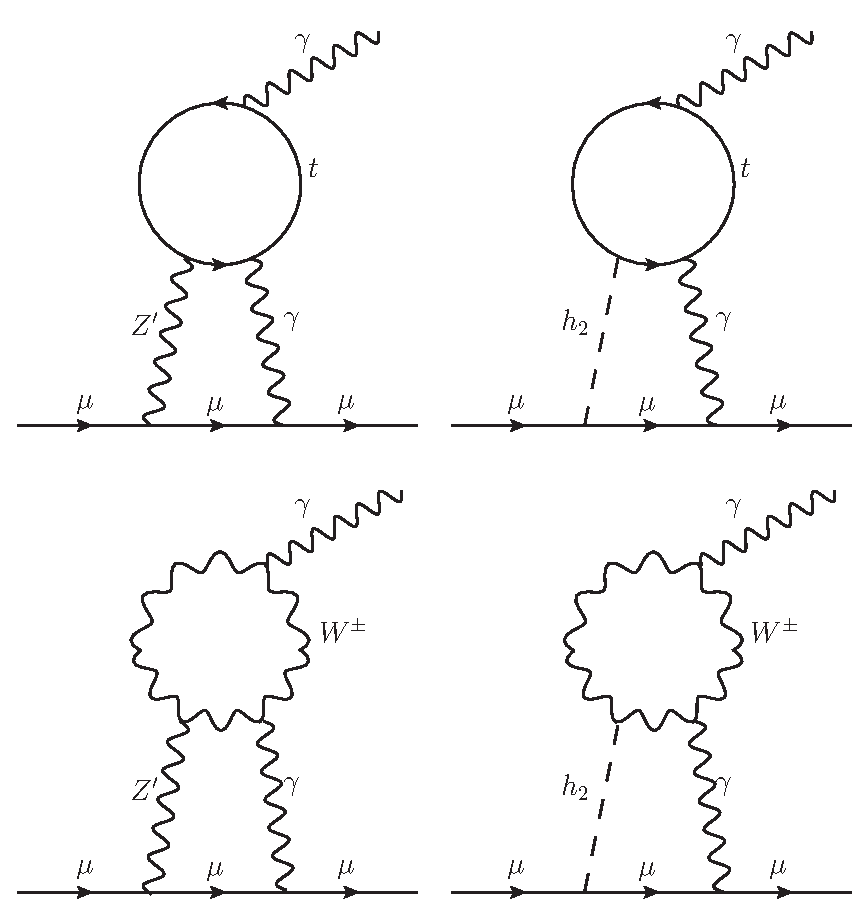
\includegraphics[scale=0.6]{/BLSM/Barr-Zee.pdf}
	\caption{Barr-Zee type two-loop diagrams contributing to $\Delta a_\mu$.}
	\label{fig:Barr-Zee}
\end{figure}	
%%%%%%%%%%%%%%%%%%%%%%%%%
The same reason that suppresses the one-loop $h_2$ contribution in Fig.~\ref{fig:g-2} is also responsible for the suppression of both the top-right and bottom-right diagrams in Fig.~\ref{fig:Barr-Zee} (for details see e.g.~Ref.~\cite{Ilisie:2015tra}). Recall that the coupling of $h_2$ to the SM particles is proportional to the scalar mixing angle $\alpha_h$, which is always small (or very small) as we can see in Fig.~\ref{fig:Plots4}. An analogous effect is present in the diagram involving a $W$-loop, where a vertex proportional to $g^{WWZ^\prime}$ suppresses such a contribution. The only diagram that might play a sizeable role is the top-left one where the couplings of $Z^\prime$ to both muons and top quarks are not negligible.

{ \color{gray}
Let us then estimate the size of the first diagram in Fig.~\ref{fig:Barr-Zee}. This type of diagrams were already calculated in Ref.~\cite{Feng:2009gn} but for the case of a SM $Z$-boson. Since the same topology holds for the considered case of B-L-SM too, 
if we trade $Z$ by the new $Z^\prime$ boson, the contribution to the muon $(g-2)_\mu$ anomaly can be rewritten as
\begin{equation}
    \Delta a_{\mu}^{\gamma Z^\prime} = -\dfrac{g^2 g^2_{\ro{B-L}} m_\mu^2 \tan^2{\theta_W}}{1536 \pi^4} \left( g_{\ro{L}}^{ttZ^\prime} - g_{\ro{R}}^{ttZ^\prime} \right) \ro{T}_7\left( m_{Z^\prime}^2, m_t^2, m_t^2 \right)\,,
    \label{eq:agZ}
\end{equation}
where $T_7$ is a loop integral. % described in appendix \ref{app:T7}. 
%
The parameters $g_{\ro{L,R}}^{ttZ^\prime}$, calculated in \texttt{SARAH}, are the left- and right-chirality projections of the $Z^\prime$ coupling to top-quarks, given by
\begin{equation}
\begin{aligned}
    g_{\ro{L}}^{ttZ^\prime} &= -\dfrac{g_{\ro{B-L}}}{3} \cos{\theta_W^\prime} + \dfrac{g}{2} \cos{\theta_W} \sin{\theta_W^\prime} - \dfrac{g_{\ro{Y}}}{6} \sin{\theta_W} \sin{\theta_W^\prime} - \dfrac{g_{\ro{YB}}}{3} \sin{\theta_W} \sin{\theta_W^\prime}\,,
    \\
    g_{\ro{R}}^{ttZ^\prime} &= -\dfrac{g_{\ro{B-L}}}{3} \cos{\theta_W^\prime} - \dfrac{2 g_{\ro{Y}}}{3} \sin{\theta_W} \sin{\theta_W^\prime} - \dfrac{g_{\ro{YB}}}{3} \sin{\theta_W} \sin{\theta_W^\prime}\,.
\end{aligned}
\end{equation}
The loop integral $\ro{T}_7 \(m_{Z^\prime}^2, m_t^2, m_t^2\)$ was determined in Ref.~\cite{Feng:2009gn} and, in the limit $m_{Z^\prime} \gg m_t$, 
%as we show in Eq.~\eqref{eq:T7-expanded}, 
it can be shown to be simplifiable to, 
\begin{equation}
    \ro{T}_7 \(m_{Z^\prime}^2, m_t^2, m_t^2\) \simeq \frac{2}{m_{Z^\prime}^2} \,,
    \label{eq:T7}
\end{equation}
up to a small truncation error. %(see Appendix~\ref{app:T7} for details).
For the parameter space region under consideration the difference $g_{\ro{L}}^{ttZ^\prime} - g_{\ro{R}}^{ttZ^\prime}$ can be cast in a simplified form as follows 
\begin{equation}
    \left(g_{\ro{L}}^{ttZ^\prime} - g_{\ro{R}}^{ttZ^\prime}\right) \simeq \dfrac{\left(g^2+g_{\ro{Y}}^2\right)g_{\ro{YB}}}{32 g_{\ro{B-L}}} \left(\dfrac{v}{x}\right)^2\,.
    \label{eq:gLminusgR}
\end{equation}
Using this result and the approximate value of the loop factor, we can calculate the ratio between 
the two- and one-loop contributions to the muon $(g-2)_{\mu}$,
\begin{equation}
    \dfrac{\Delta a_{\mu}^{\gamma Z^\prime}}{\Delta a_{\mu}^{Z^\prime}} \simeq -\dfrac{g^2 g_{\ro{Y}^2}}{2048 \pi^2} \dfrac{g_{\ro{YB}}}{g_{\ro{B-L}}} \left( \dfrac{v}{x} \right)^2 \ll 1\,,
\end{equation}
which shows that $\Delta a_\mu^{\gamma Z^\prime}$ does indeed play a subdominant role in our analysis and can be safely neglected. } 


%\chapter{3HDM}
\label{ch:3HDM}


%\renewcommand{\cleardoublepage}{}
\renewcommand{\clearpage}{}

\chapter{Conclusions}
\label{ch:Conclusions}

%\section{The B-L-SM Conclusions}
%\label{sec:Conclusions BLSM}

%  
%
%Although this is the basis of the work presented here a effort was made to incorporate new machine learning routines via the initial building of smaller learning sets by conventional methods. 
%
%

To summarize, in this thesis we have performed a detailed phenomenological analysis of the minimal $\U{B-L}$ extension of the Standard Model known as the B-L-SM and the a BGL-like 3HDM with a $\mathrm{U(1)} \times \mathbb{Z}_2$ symmetry. 
%
This phenomenological analysis was produced by a set of tools developed as to be easily adaptable to fit new models. 

Note, although we use conventional means to perform this analysis, some modern studies have incorporated new strategies to scan these complex problems like machine learning. Similar to done by our colleagues in \cite{freitas2020phenomenology}. These new methods promise to greatly increase the efficacy of similar studies. 
%
Unfortunately this wasn't accomplished in this work due to the exceptional setbacks. A feature of this year, that affected partially the quality of the work. 
%
These machine learning routines could reveal much faster


In the B-L-SM (chapter \ref{Chap:B-L-SM_Model}), we have confronted the model with the most recent experimental bounds from the direct $Z^\prime$ boson and next-to-lightest Higgs state searches at the LHC.
%
Simultaneously, we have analysed the prospects of the B-L-SM for a consistent explanation of the observed anomaly in the muon anomalous magnetic moment $(g-2)_{\mu}$. 
%
Done by exploring the B-L-SM potential for the observed $(g-2)_{\mu}$ anomaly in the regions of the model parameter space that are consistent with direct searches and EW precision observables.

As one of the main results of our analysis, we have found phenomenologically consistent parameter space regions that simultaneously fit the exclusion limits from direct $Z^\prime$ searches and can explain the muon $(g-2)_{\mu}$ anomaly. 
%
We have distinguished four benchmark points for future phenomenological exploration at experiments, the first one with the lightest allowed $Z^\prime$ ($m_{Z^\prime}>3.1$ TeV), the second with the lightest additional scalar boson ($m_{h_2}>400$ GeV), and the other two points that reproduce the muon $(g-2)_{\mu}$ anomaly within $1\sigma$ uncertainty range. 
%
Besides, we have studied the correlations of the $Z^\prime$ production cross section times the branching ratio into a pair of light leptons versus the physical parameters of the model.
%
In particular, we have found that the muon $(g-2)_{\mu}$ observable dominated by $Z^\prime$ loop contributions lies within the phenomenologically viable parameter space domain. 
%
For completeness, we have also estimated the dominant contribution from the Barr-Zee type two-loop corrections and found a relatively small effect.

%%%%%% 

As for the 3HDM portion of our work in this these seen in  Chapter\,\ref{ch:3HDM}. 
%
We verified the phenomenological consistency of our model, we identified a region where both flavour and scalar sector physics are within experimental bounds including, like in the B-L-SM, EW precision observables and direct detection bounds.  
%
%We noted that there is a large region of the paramater space that is consistent with flavour QFV observables and where they are not respected. 
%
Narrowing down consistent the parameter space regions that simultaneously fit the exclusion limits from direct scalar searches and flavour constraints. 

For this we determined the most sensitive flavour violation channels, and concluded that the stabilizing flavour symmetry is a mechanism that allows the model to be consist with current flavour observations. 
%
We also propose that further deviations in these flavour observables might be a pathway as to discover Higgs boson (or other exotic particle) mediating these phenomena. 
%
Being that the most appropriate channels to peer into this could be B meson oscillations and B meson decays for this type of 3HDM.

However a key take away from our results we show that the most stringent constraint on the model is not the flavour observables but the Higgs physics limits. 
%
A significant conclusion seeing that new upgrades at the LHCb, Belle and Atlas experiments could mean that despite the flavour sector being constraint the lightest possible Higgs might soon be in the TeV range. 

We recognize these conclusions might not be sufficient to fully examine the model since there might be room for a wider paramater space if exact alignment is not performed or if loop order effects are allowed.

In our study of the 3HDM we have highlighted six benchmark points to illustrate how low masses are still within the range of future colider experiments.

% {\color{blue} I am unsure what to add } 

%We have distinguished four benchmark points for future phenomenological exploration at experiments, the first one with the lightest allowed $Z^\prime$ ($m_{Z^\prime}>3.1$ TeV), the second with the lightest additional scalar boson ($m_{h_2}>400$ GeV), and the other two points that reproduce the muon $(g-2)_{\mu}$ anomaly within $1\sigma$ uncertainty range. 

%Especially if this mixing comes from light scalars. 
%
%Note that we found that there are exotic scalars with very light masses that sucessful pass all constraints. 
% 
%This study might pave the way for continued work in direct scalar searches. 

%T some of the allowed exotic scalars are found to be light indicating that the model succeeds in confronting flavour data even in the presence of scalars as lightas 300 GeV. Hence, the studied 3HDM opens the door to direct searches for non-SM scalarsat future runs of the LHC.

%As for the 3HDM presented in Chapter\,\ref{ch:3HDM}. 
%
%Our numerical analysis show that a 3HDM Model when stabilized trough a flavour symmetry that is softly broken can provide a way to suppress the appearance of tree-level FCNCs. 
%
%Although these FCNCs mediated by the scalar fields have NP contributions that can be sizable, but are not when scalar scattering is considered. 
%
%We also discuss that there are stronger constraints on the model coming from it's enlarged scalar sector.
%

%\section{ Future Work}



%% \chapter{Appendix}

\newpage 

\section{Appendix}

\subsection{Gamma Matrices}
The $\gamma$ matrices are defined as, 
\begin{equation}
\{  \gamma^\mu , \gamma^\nu \} = 2 g^{\mu \nu} I 
\end{equation}
where, 
\begin{equation}
g^{ \mu \nu } = 
\begin{pmatrix}
1 & 0 & 0 & 0 \\
0 & -1 & 0 & 0  \\
0 & 0 & -1 & 0 \\
0 & 0 & 0 & -1 \\
\end{pmatrix}
\end{equation}
and if $\gamma_\mu = (\gamma^0, \gamma)$  then it is usual to require for the hermitian conjugate matrices,
\begin{equation}
\gamma^{0 \dagger} = \gamma^0 \quad \textrm{and} \quad \gamma^\dagger = - \gamma 
\end{equation}


\subsection{Lagrangian Dynamics}

In Lagrangian dynamics we define the action $S$ has, 
\begin{equation}
\mathcal{S} = \int L \, dt = \int \mathcal{L}(\phi,\partial \phi ) \, d^4x  
\end{equation}
where $L$ is the Lagrangian, and the $\mathcal{L}$ is designated as the \textit{Lagrangian density}, note these terms are
usually used interchangeable. Here $\mathcal{L}$ is a function of the field $\phi$ and it's spatial derivatives. 

The action $S$ is constrained by the principle of least action, this requires the "path" taken by a field between an initial and final set
of coordinates to leave the action invariant, this can be expressed by,
\begin{equation}
\partial \mathcal{S} = 0 
\end{equation}
from here one can deduce the \textit{Euler-Lagrange} equations,
\begin{equation}
\partial_\mu \left( \frac{\partial \mathcal{L}(\phi,\partial \phi ) }{ \partial (\partial_\mu) } \right) - \frac{ \partial \mathcal{L}(\phi,\partial \phi ) }{ \partial \phi }  = 0 
\end{equation} 


\bibliography{bib.bib}
\bibliographystyle{ieeetr}

\end{document}
